\chapter{\uppercase{Active Trusses}}  
\label{section:chap_05_active_trusses} 
Simulations of shape changing in active truss structures are discussed in this chapter. Finite element analyses of 3D truss system are presented and both material and geometric nonlinearities are considered in the analyses. Two truss systems with cubical and tetrahedral arrangements of trusses as building blocks are considered in order to generate planar truss and longitudinal (beam like) truss systems, respectively. Shape changing in these truss systems is controlled by an actuation of each truss component using a piezoelectric actuation.

\section{Deformed Shapes}  
\label{section:chap_05_1_deformed_shape_of_truss}
Consider a 3D continuum object in a reference configuration $X_i$.
This continuum object changes its shape from the reference $X_i$ configuration to current configuration $x_i$.
In the case of Lagrangian description, the current configuration is defined as a function of reference configuration:

\begin{equation}  
x_i=\chi (X_i)   
\label{lagrangian_descriptoin} 
\end{equation}
Since the new configuration is decided a priori, the mapping function $\chi (X_i)$ is defined and the gradient of deformation is known:
\begin{equation}
F_{ij}=\frac{\partial x_i}{\partial X_j}
\label{deformation_gradient_tensor}
\end{equation}
The strain corresponding to the induced deformation in the truss system is easily calculated.  
The Green-St. Venant strain is given as:
\begin{equation}
E_{KL}=\frac{1}{2}\left( \frac{\partial x_j}{\partial X_K}\frac{\partial x_j}{\partial X_L}-\delta_{KL}\right)
\label{lagrange_green_strain}
\end{equation}
In order to induce the desired strain in each truss member associated with the shape change, an electric field is prescribed to the truss member. The deformation in each truss member is considered only along the longitudinal axis of each truss. Thus, strain transformation from the global coordinate to the local orientation of each truss member is needed in order to determine amount of strain in the longitudinal axis of each truss. Discussion on the strain transformation is presented below. Once the amount of longitudinal strain for each member has been determined, the constitutive relation is used in order to calculate the magnitude and direction of external stimuli that should be prescribed: 
\begin{equation}
E_{11}=f_1(S_{11})+f_2(E_3)
\label{one_constitutive_equation}
\end{equation}
where $E_{11}$ is the axial strain along the longitudinal axis of each truss member, $f_1(S_{11})$ is the strain due to the mechanical stress along the longitudinal axis of the truss $S_{11}$ and $f_2$ is the strain due to the electric field input, prescribed through the thickness of the truss, $E_3$.
In order to achieve desired shapes in the truss system, either stress or electric field, or both stress and electric field can be prescribed.
\section{Nonlinear Truss Finite Element}
Truss systems consist of relatively slender members connected by pin joints.
The pin joints allow the members to rotate with respect to each other.
Each truss element is specified by two joints in the space and the shortest distance connects these two joints.
Let us consider two joints $P_1$ and $P_2$.
The locations of these two joints in the reference configuration are defined by two vectors namely $\mathbf {X^{P_1}}$ and $\mathbf {X^{P_2}}$.
The vector that connects these two joints in the reference configuration is defined as:
\begin{equation}
\mathbf {V^{12}=X^{P_2}-X^{P_1} } 
\end{equation}
and the base vector in the longitudinal direction of each truss member that connects these two joints is: 
\begin{equation}
\mathbf {N^{12}=V^{12}/ \|V^{12}\| }
\label{base_vector_definition}
\end{equation}
The base vector in the longitudinal direction of each truss member $\mathbf {N^{12}}$ is used to define a transformation matrix between local and global coordinates.
The longitudinal strain in each truss member is related to the global strain of the truss system by a transformation $ \mathbf {Q}=\mathbf {N^{12}} \otimes \mathbf{N^{12} }$. 
This transformation is used to determine the magnitude of strain along the longitudinal axis of the truss.
The constitutive relation for the truss is discussed later in this chapter.

The displacement in the truss systems is defined in terms of a displacement of each node with respect to the reference configuration: 
\begin{equation}
u^{P_1}_i=x^{P_1}_i-X^{P_1}_i ; u^{P_2}_i=x^{P_2}_i-X^{P_2}_i ;  
\end{equation}
If linear test functions are used for the finite element approximation, the displacement at each point on the truss can be interpolated as a linear function. The same shape function is used to interpolate the geometry of the truss. The master shape function of the isoparametric element $\zeta \in [-1,1]$ is introduced as:
\begin{equation}
\begin{aligned}
& \psi^1=0.5(1+\zeta); \psi^1_{,\zeta}= 0.5 \\
& \psi^2=0.5(1-\zeta); \psi^2_{,\zeta}=-0.5
\end{aligned}
\label{shape_function_truss} 
\end{equation}
The mapping must be defined from each truss element into this master element.
The global deformation gradient is:
\begin{equation}
\frac{\partial u_i}{\partial X_j}=\frac{\partial u_i}{\partial \zeta}
\frac{\partial \zeta}{\partial X_j}
\label{eqn:global_derivitave} 
\end{equation}
For the truss element in 3D the gradient of deformation is:
\begin{equation}
\frac{\partial X_j }{\partial \zeta}= 
  \sum_{i=1}^{NPE=2} \psi^i_{,\zeta} X^{P_i}_j 
\label{eqn:delXi_delzeta} 
\end{equation}
where NPE is the number of joints in an element.
It is noted that the integration is done on the member that connects two joints of the truss element.
Then the deformation gradient at a point on the truss is defined as:
\begin{equation}
F_{ij}=\delta_{ij}+ \frac{\partial u_i}{\partial X_j};  
\end{equation}

\subsection{Space Filler Truss Configuration}
The first example considered is a planar truss. 
The truss is formed by cubical elements. Figure \ref{fig:cuber_space_filler_truss} provides an example for one of these elements. 
Each of the elements consists of 12 side and 4 diagonal truss members. Deformation of the members can be controlled by various stimuli, including electric fields. 
Changes in the length of each member will cause change of shape of each single cubical element and consequently change in shape of the structure that is made of these members.

\begin{figure} 
\centering
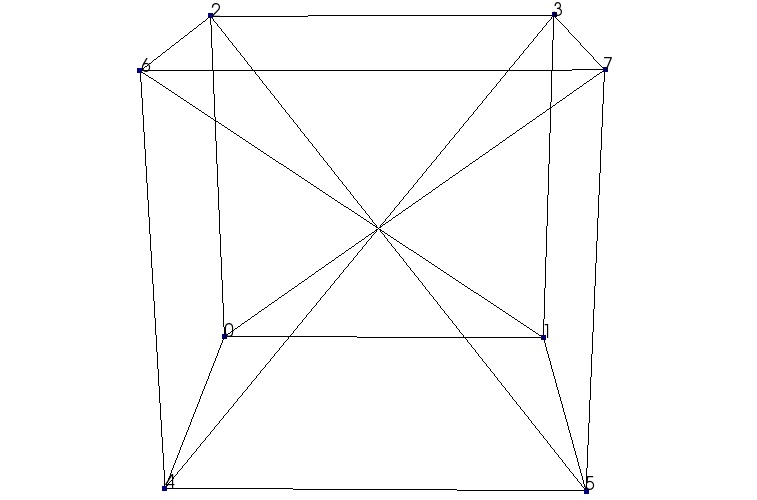
\includegraphics[width=6.0in]{./chap_5_active_trusses/images_space_filler/cube.png}
\caption{One element of space filler truss}
\label{fig:cuber_space_filler_truss}
\end{figure}

As an example, consider a planar domain that is in the form of a plate structure.
The domain is defined as follows: 

\begin{equation} 
\begin{aligned}
X_1 \in & [-L_1/2,L_1/2] \\
X_2 \in & [-L_2/2,L_2/2] \\
X_3 \in & [-h/2,h/2]
\end{aligned}
\label{planar_truss_domain:eqn}
\end{equation}
 
Let us first consider $[L_1,L_2,h]=[1,1,0.1]$ unit is in meter, and fill the domain with 20x20 elements in $X_1$ and $X_2$ directions and 1 element in $X_3$ direction. 
The planar truss is shown in figure \ref{fig:planar_truss_ref_config}.  
If the truss system is intended to have a shape as is shown in figure \ref{fig:xy_plane_desired_shape} the mapping between the reference and current configurations for $X_3=X_1 X_2$ surface is defined as follows.

\begin{equation}
\begin{aligned}
x_1(X_1,X_2,X_3) = & X_1 \\
x_2(X_1,X_2,X_3) = & X_2 \\
x_3(X_1,X_2,X_3) = & X_3+X_1 X_2 \\
\end{aligned}
\label{doubly_curved_mapping:eqn}
\end{equation}
The deformation gradient for this above mapping function is defined as:
\begin{equation}
\mathbf F=
\begin{bmatrix}
1&0&0 \\
0&1&0 \\
X_2 & X_1 & 1
\end{bmatrix}
\label{deformation_gradient_doubly_curved_mapping:eqn}
\end{equation}
Then the stretch tensor $\mathbf C=\mathbf {F^T F}$ and Green-St. Venant strain tensors are:
\begin{equation}
\mathbf C=
\begin{bmatrix}
X_{2}^2+1&X_{1}\,
X_{2}&X_{2}\cr X_{1}\,X_{2}&X_{1}^2+1&X_{
 1}\cr X_{2}&X_{1}&1\cr 
\end{bmatrix}
; \mathbf E=
\begin{bmatrix}
X_{2}^2&X_{1}\,X_{2}&X_{2}\cr X_{1}\,X_{2}&X_{1}^2&X_{1}\cr X_{2}&X_{1}&0\cr 
 \end{bmatrix}
\label{green_deformation_tensor_doubly_curved_mapping:eqn}
\end{equation} 
The transformation from the above-calculated strain to the local strains along the longitudinal axes for all members in the truss system is done by $\mathbf E^{truss}=\mathbf E \cdot \mathbf {Q}$. The transformation matrix is obtained from the base vector of each truss and is discussed in the previous section.

\begin{figure} 
\centering
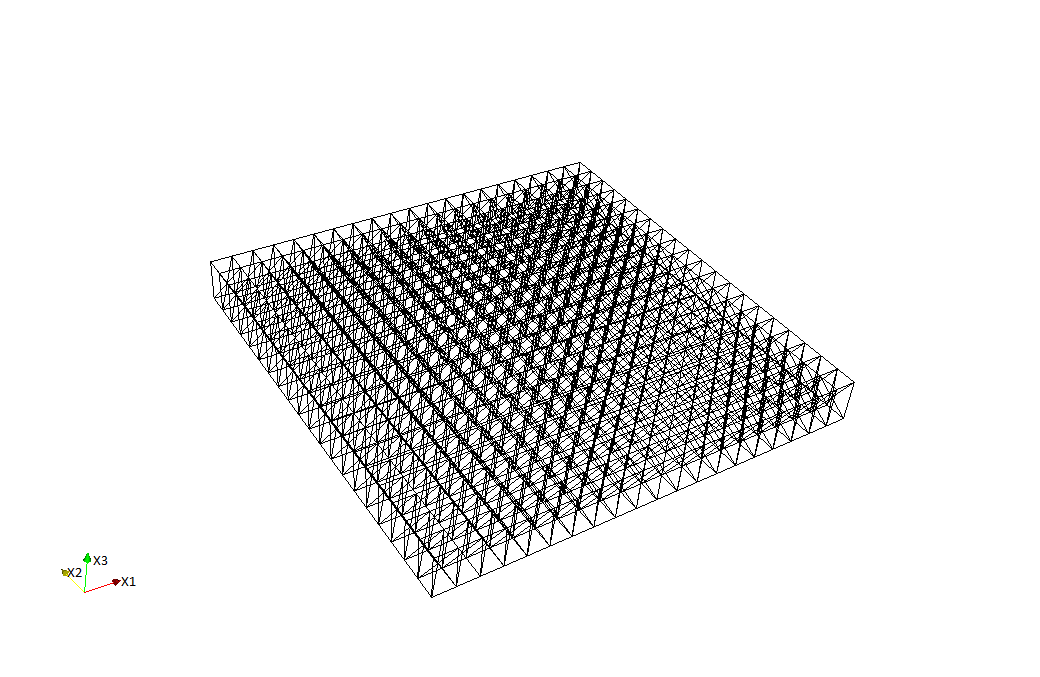
\includegraphics[width=6.0in]{./chap_5_active_trusses/images_space_filler/planar_truss_ref_config.png}
\caption{Planar truss in reference configuration}
\label{fig:planar_truss_ref_config}
\end{figure}

\begin{figure} 
\centering
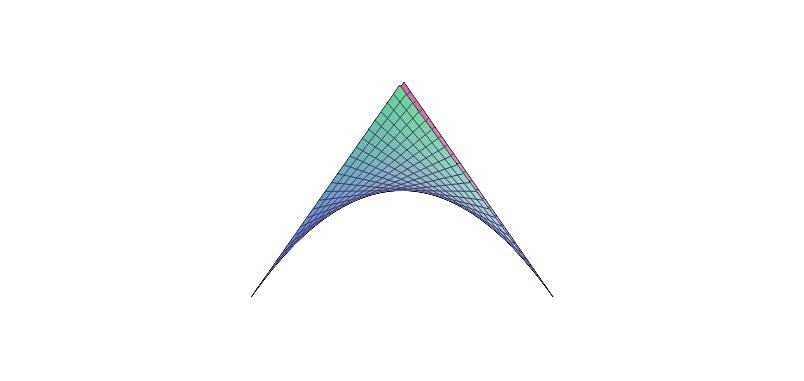
\includegraphics[width=6.0in]{./chap_5_active_trusses/images_space_filler/xy_plane_desired_shape.jpg}
\caption{The desired current configuration for the planar truss}
\label{fig:xy_plane_desired_shape}
\end{figure}

\begin{figure} 
\centering
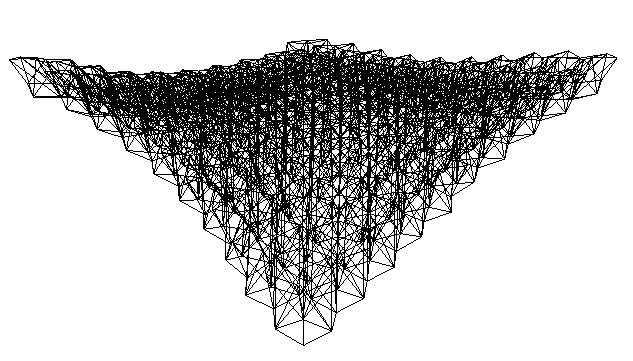
\includegraphics[width=4.5in]{./chap_5_active_trusses/images_space_filler/planar_truss_deformed_config_shape.png}
\caption{Shape changing in the planar truss} 
\label{fig:planar_truss_deformed_config}
\end{figure}


\begin{figure} 
\centering
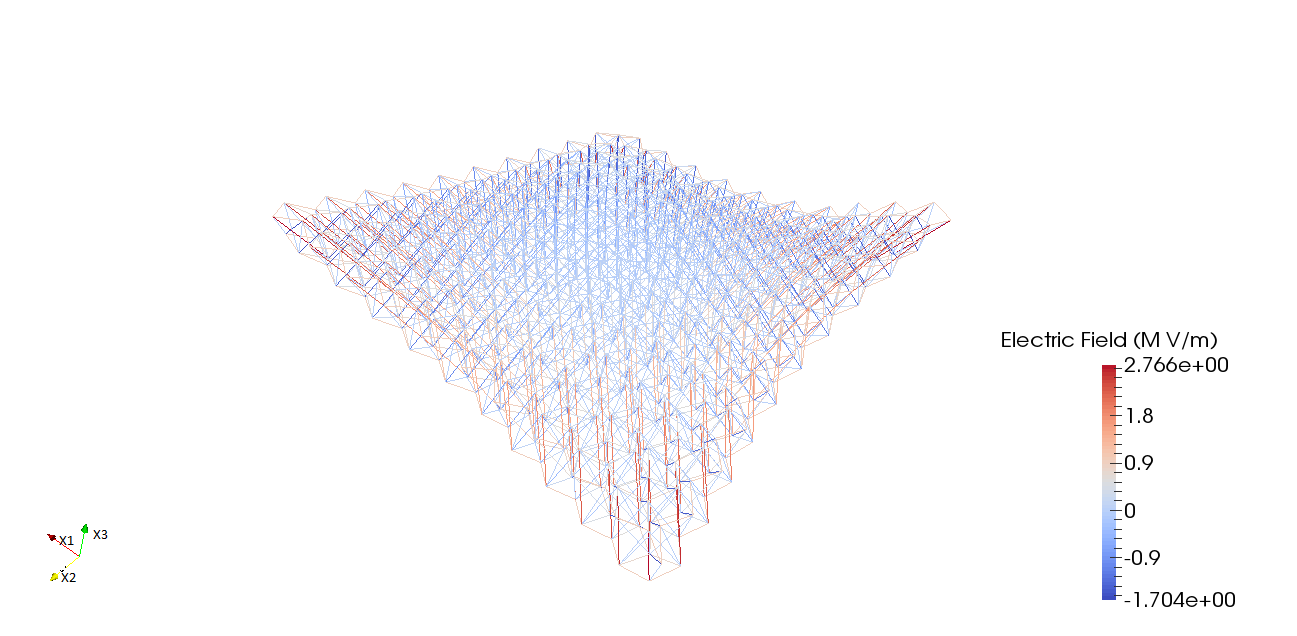
\includegraphics[width=6.0in]{./chap_5_active_trusses/images_space_filler/planar_truss_deformed_efield_z_eq_xy.png}
\caption{The deformed configuration for the planar truss under electric field} 
\label{fig:planar_truss_deformed_config_efield}
\end{figure}

In order to induce the shape changes shown in figure \ref{fig:xy_plane_desired_shape}, electric field is prescribed to each truss members. To determine the amount of strains along the longitudinal axes of the truss members, the strain tensor given in equation (\ref{green_deformation_tensor_doubly_curved_mapping:eqn}) is transformed to the local orientation for the truss members following the strain transformation in Section \ref{section:chap_05_1_deformed_shape_of_truss}. Figure \ref{fig:planar_truss_deformed_config} shows the deformed shape of the planar truss due to applications of electric field, and the amount of electric field prescribed in shown in figure \ref{fig:planar_truss_deformed_config_efield}. Linear electro-mechanical constitutive relation is considered and the following piezoelectric constant is used $d_{311}^0 = 340pm∕V$. It is seen that the amount of electric field required to activate the truss is high, which might be beyond the tolerance of the materials. The main reason is due to the use of linear electro-mechanical relation for the piezoelectric materials. It will be shown later, when a nonlinear constitutive relation is considered, shape changes in the truss systems can be achieved with reasonable values of electric field input, which is within the operating condition of piezoelectric ceramics. 

It is shown in figure \ref{fig:planar_truss_deformed_config_efield} that the application of electric stimuli to each truss member can induce desired shape. The space filler truss that has been discussed in the previous chapter can offer good flexibility for planar shapes. 

Another shape that is considered for the planar truss is the saddle point surface. The shape $X_3=X_1^2-X_2^2$ is induced in the planar truss with the same procedure that is already described. 



The strain induced in each truss for this truss configuration in shown in figure \ref{fig:planar_z_eq_x2_y2_strain_contour}.  If we assume that truss member are made of electro active materials with overall electromechanical coupling coefficient as $d_{311}^0=340pm/V$. The corresponding required electric field contour for each truss will be as in figure \ref{fig:planar_z_eq_x2_y2_efield_contour}. 

% If we assume that truss member are made of electro active materials with overall electromechanical coupling coefficient as $d_{311}^0=340pm/V$. 
% The corresponding required electric field contour for each truss will be as in figure \ref{fig:planar_z_eq_x2_y2_efield_contour}.
% The strain induced in each truss for this truss configuration in shown in figure \ref{fig:planar_z_eq_x2_y2_strain_contour}.

\begin{figure} 
\centering
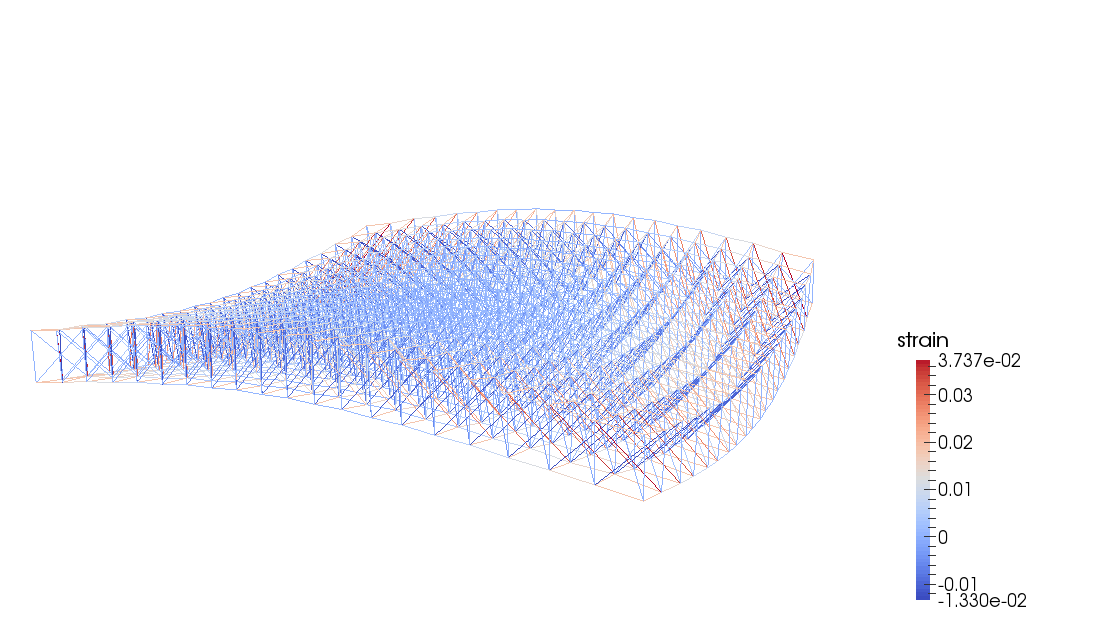
\includegraphics[width=6.0in]{./chap_5_active_trusses/images_space_filler/planar_truss_z_eq_x2_y2_strain.png}
\caption{The strain contour of planar space filler truss for the $X_3=X_1^2-X_2^2$ shape (displacement are scaled 20 times)}
\label{fig:planar_z_eq_x2_y2_strain_contour}
\end{figure} 

\begin{figure} 
\centering
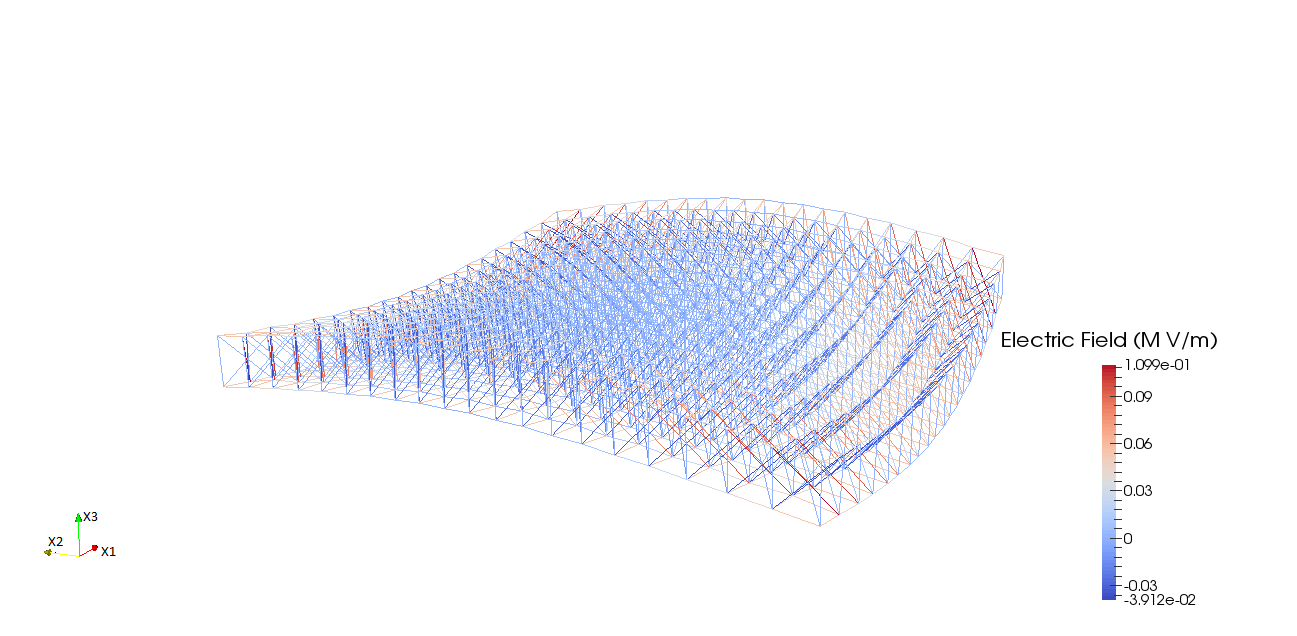
\includegraphics[width=6.0in]{./chap_5_active_trusses/images_space_filler/planar_truss_z_eq_x2_y2_elec_field.png}
\caption{The electric field contour of planar space filler truss for the $X_3=X_1^2-X_2^2$ shape (displacement are scaled 20 times)}
\label{fig:planar_z_eq_x2_y2_efield_contour}
\end{figure} 

\subsection{Tetrahedral Beam Like Truss}
Using a tetrahedral shape as a building block for truss configurations it is possible to form the longitudinal truss elements to take a beam like form. The building block of the tetrahedral beam like truss is shown in figure \ref{fig:building_block_of_tetrahedral_truss} that contains 3 tetrahedral. 


The beam like truss is formed by arranging these tetrahedral units in one direction. An example of truss with 150 tetrahedral units is shown in figure \ref{fig:refrence_shap_100_tetra_unit_tetrahedral_unit}. 
\begin{figure} 
\centering
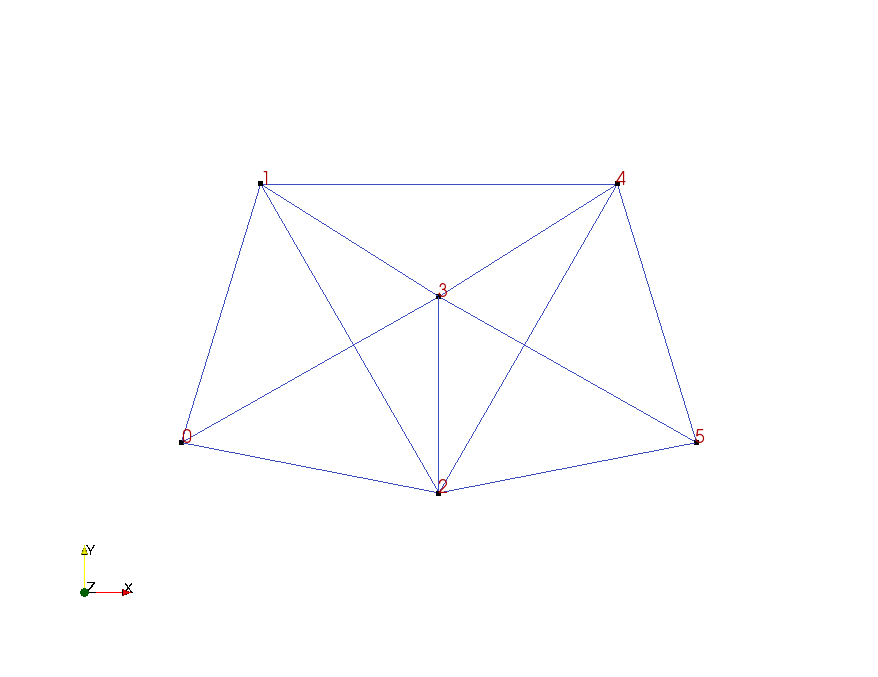
\includegraphics[width=6.0in]{./chap_5_active_trusses/images_linear_tetrahedral/building_block_of_tetrahedral_truss.png}
\caption{The building block of tetrahedral beam like truss}
\label{fig:building_block_of_tetrahedral_truss}
\end{figure} 

\begin{figure} 
\centering
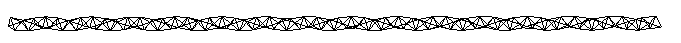
\includegraphics[width=6.0in]{./chap_5_active_trusses/images_linear_tetrahedral/refrence_shap_100_tetra_unit_tetrahedral_unit.png}
\caption{Tetrahedral beam like truss with 150 units that is used as reference configuration}
\label{fig:refrence_shap_100_tetra_unit_tetrahedral_unit}
\end{figure} 
It can be seen form the cross section view of the beam in figure \ref{fig:refrence_shap_100_tetra_unit_tetrahedral_unit_cross_section_view} that none of the truss members crosses the center line. Therefore, this configuration behaves like a hollow beam. Several examples of bending deformations are considered for the truss system. The bending can be induced by creating normal strain in the axial direction of the truss members along the longitudinal axis of the beam. In the simple bending case and disregarding the thought thickness shear of the beam, along the axis normal strain of the beam is defined with respect to the radius of curvature of the beam $r_{curvature}$:

\begin{equation}
\begin{aligned}
r_{curvature}&=\frac{ L_{beam} }{2 \theta}\\
E_{11}&=X_3/r_{curvature}
\end{aligned}
\label{stran_and_radios_of_curvture_of_beam:eqn}
\end{equation}
where $X_3$ is the direction normal to the longitudinal axis of the beam like truss and $X_1$ is defined along longitudinal axis of the beam like truss. The remaining strain components are taken as zero.
\begin{figure} 
\centering
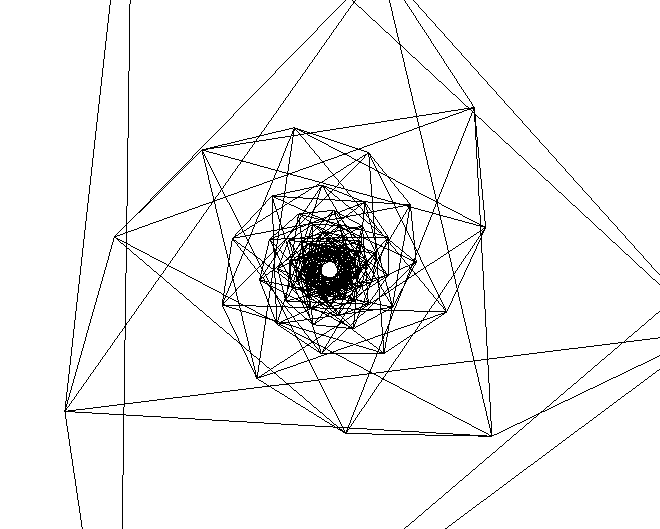
\includegraphics[width=6.0in]{./chap_5_active_trusses/images_linear_tetrahedral/refrence_shap_100_tetra_unit_tetrahedral_unit_cross_section_view.png}
\caption{Cross section view of tetrahedral beam like truss (perspective view)}
\label{fig:refrence_shap_100_tetra_unit_tetrahedral_unit_cross_section_view}
\end{figure}
$\theta$ is the curvature angle (for full circle it is $2\pi$) and
$ L_{beam}$ is the length of the beam made of tetrahedral units.
The strain $E_{11}=X_3/r_{curvature}$ causes lateral deformation in the $X_3$ direction with positive curvature.

We try to produce the shape of an arc with a curvature angle $\pi$. The result is shown is figure \ref{fig:tetra_hedral_arc_pi_shape}. As can be seen the shape is quite different from the real arc. The reason of the difference between the produced shape and desired shape is due to disregarding the normal strain in the thickness direction of beam that is produced in bending of a beam. Increasing the curvature in the tetrahedral beam like truss will cause a sinusoidal like shape in the truss as it is shown in figure \ref{fig:tetra_hedral_arc_2_pi_shape}. The strain that is induced in this truss is taken from equation (\ref{stran_and_radios_of_curvture_of_beam:eqn}) with $\theta=2 \pi$.

\begin{figure} 
\centering
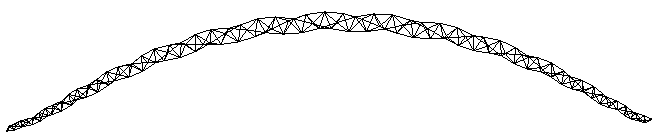
\includegraphics[width=6.0in]{./chap_5_active_trusses/images_linear_tetrahedral/tetra_hedral_arc_pi_shape.png}
\caption{Arc shape produced in the tetrahedral beam like truss}
\label{fig:tetra_hedral_arc_pi_shape}
\end{figure}  


\begin{figure} 
\centering
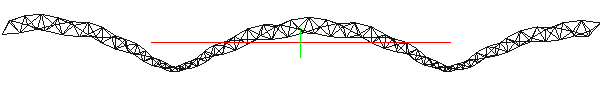
\includegraphics[width=6.0in]{./chap_5_active_trusses/images_linear_tetrahedral/tetra_hedral_arc_2_pi_shape.png}
\caption{Cyclic shape produced in the tetrahedral beam like truss}
\label{fig:tetra_hedral_arc_2_pi_shape}
\end{figure} 


In order to get a shape closer to the actual bending of a beam we then apply the normal strain in the thickness direction. This will cause a strain of the field closer to the strain beam made of continuous solid members. We modify the bending strain defined in equation (\ref{stran_and_radios_of_curvture_of_beam:eqn}) with the through thickness normal strain as follows: 

\begin{equation}
\begin{aligned}
E_{11}&=X_3/r_{curvature}+\kappa_v \\
E_{22}&=-X_3/(2r_{curvature})+\kappa_v \\
E_{33}&=-X_3/(2r_{curvature})+\kappa_v
\end{aligned}
\label{strain_with_dilation:eqn}
\end{equation}
where $\kappa_v$  is the dilation that is added to mimic the effect of change in volume in the beam. The remaining strain components are taken as zero. It is observed that if $\kappa_v=2.0$ there will be an arc forming in the beam like truss. This arc is shown in figure  \ref{fig:tetra_hedral_arc_2_pi_shape_with_pressure}. 

\begin{figure}  
\centering
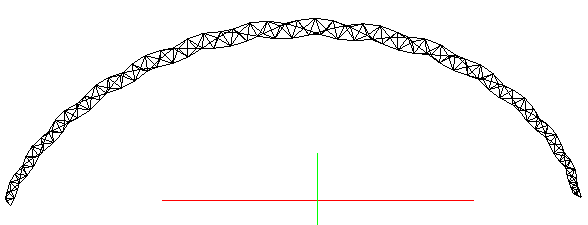
\includegraphics[width=6.0in]{./chap_5_active_trusses/images_linear_tetrahedral/tetra_hedral_arc_2_pi_shape_with_pressure.png}
\caption{Shape produced in the tetrahedral beam like truss including the all normal strains}
\label{fig:tetra_hedral_arc_2_pi_shape_with_pressure}
\end{figure} 

In the last example we will try to apply a shape in the beam in the way that it passes four specific points. Consider bending of a tetrahedral beam like truss in the way that it passes through three points as follows: 
\begin{equation}
\begin{aligned} 
\underline X ^1&=(0,0,0) \\
\underline X ^2&=(L_{beam}/4,0,L_{beam}/8) \\
\underline X ^3&=(3 L_{beam}/4,0,-L_{beam}/8) \\
\underline X ^4&=(L_{beam},0,L_{beam}/8)
\end{aligned}
\label{three_points:eqn}
\end{equation}

In this case it can be found that the following strain should be applied, the remaining strain components are taken as zero: 

\begin{equation}
E_{11}=X_3 \left(
\frac{329}{36L_{beam}} -
\frac{220 X_1}{L_{beam}^2} +
\frac{280 X_1}{ 3 L_{beam}^3}  \right)
\label{three_points_strain:eqn}
\end{equation}

The desired shape and the final shape of the linear truss the case that it passes through three specific points as are shown in figure \ref{fig:tetra_hedral_three_point}.

\begin{figure}
\centering
\fbox{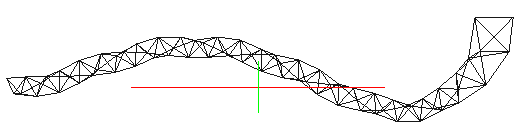
\includegraphics[width=6.0in]{./chap_5_active_trusses/truss_image_three_point/current_tetra_beamthree_point}}
\fbox{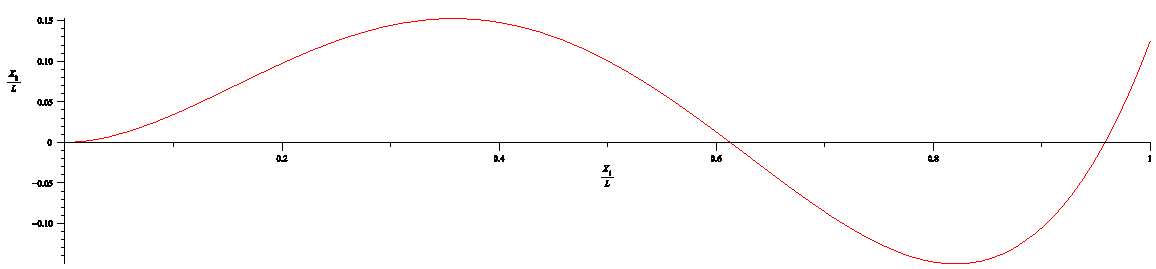
\includegraphics[width=6.0in]{./chap_5_active_trusses/truss_image_three_point/curve_beam-eps-converted-to_three_point}}
\caption{Shape of tetrahedral beam that passes through four specific points}
\label{fig:tetra_hedral_three_point}
\end{figure}

\subsection{Effect of Nonlinear and Time Dependent Constitutive Equation on Active Truss}
By prescribing the above calculated strain field to the truss structure, the desired shape is attained. The corresponding strain in each truss element is achieved through applications of electric field to the piezoelectric materials in the truss members.
In the case of piezoelectric patch with the electro-mechanical coupling factor $d_{311}$ the electric field that should be applied to each truss $E_3$ can be found from the following equation:

\begin{equation}
\begin{aligned}
E_{11}^{truss} &=\sum_{i=1}^3 \sum_{j=1}^3 E_{ij}N^{truss}_i N^{truss}_j\\
E_{11}^{truss} &=E_3 d_{311} 
\end{aligned}
\label{electric_field_in_each_truss:eqn}
\end{equation}
where 
$N^{truss}_{i}$ are the componenst of the base vector in the longitudinal direction of each truss member $\mathbf {N^{12}}$ that is defined in equation (\ref{base_vector_definition}).
$E_3$ is the electric field that should be applied to each truss element to induce the deformation.
When a nonlinear electro-mechanical constitutive equation is considered, the strain in the longitudinal axis of each truss is a nonlinear equation.
The relationship between the strain and electric field can also be taken as time dependent to include hystersis response of piezoelectric materials.

The effect of nonlinear and time dependent electro-mechanical response of each truss member on the overall deformation of truss structure is examined.
The time dependent constitutive equation based on quasi linear viscoelastic model that was introduced in previous chapters is used.
The tetrahedral truss system is used for these analyses and the desired shape is taken to be an arc with arc angle of $\pi/2$.
The strain distribution for this configuration is shown in figure \ref{fig:linear_tetrahedral_bending_strain_contour}.
\begin{figure} 
\centering
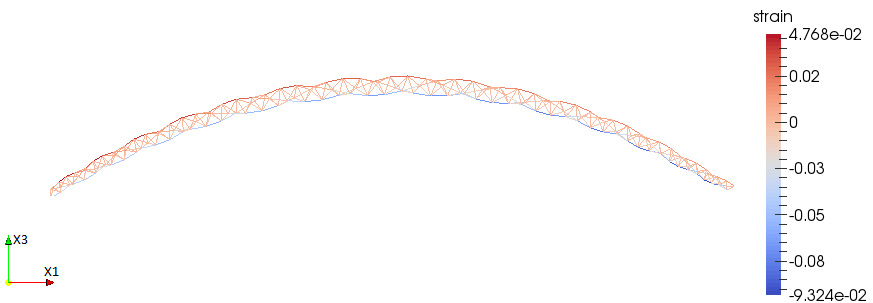
\includegraphics[width=6.0in]{./chap_5_active_trusses/images_non_linear_time_dependent_constitutive_equatio/linear_tetrahedral_bending_strain_contour.png}
\caption{The strain distribution in a beam like tetrahedral truss in the arc configuration}
\label{fig:linear_tetrahedral_bending_strain_contour}
\end{figure} 
If we take the electromechanical coupling factor as $d_{311}^0=340pm/V$ the corresponding required electric field contour for each truss shape is shown in figure \ref{fig:linear_tetrahedral_bending_efield_contour}.

\begin{figure} 
\centering
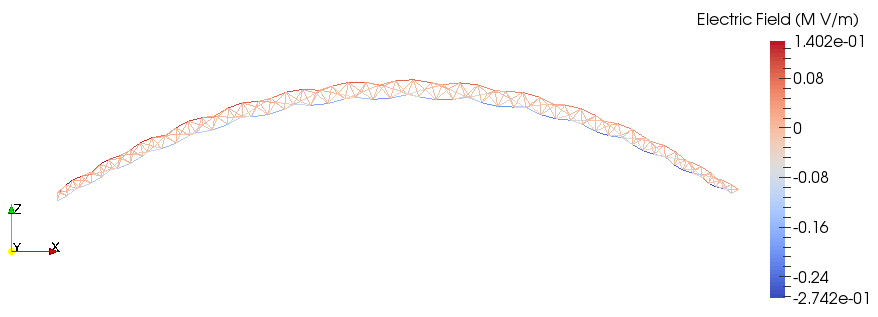
\includegraphics[width=6.0in]{./chap_5_active_trusses/images_non_linear_time_dependent_constitutive_equatio/linear_tetrahedral_bending_electric_field_contour.png}
\caption{The electric field distribution in a beam like tetrahedral truss in the arc configuration}
\label{fig:linear_tetrahedral_bending_efield_contour}
\end{figure} 

At first the analyses is conducted for a linear constitutive model for the truss.
The coupling between the stimuli and strain in the truss members are taken to be linear and independent of time.
The relationship between the input stimuli and maximum deflection in the middle of beam like tetrahedral beam in this analyses is shown in figure \ref{fig:linear_static_stimuli_vs_displacement}.
The stimulus is applied to each truss member with the frequency of 1Hz.
\begin{figure} 
\centering
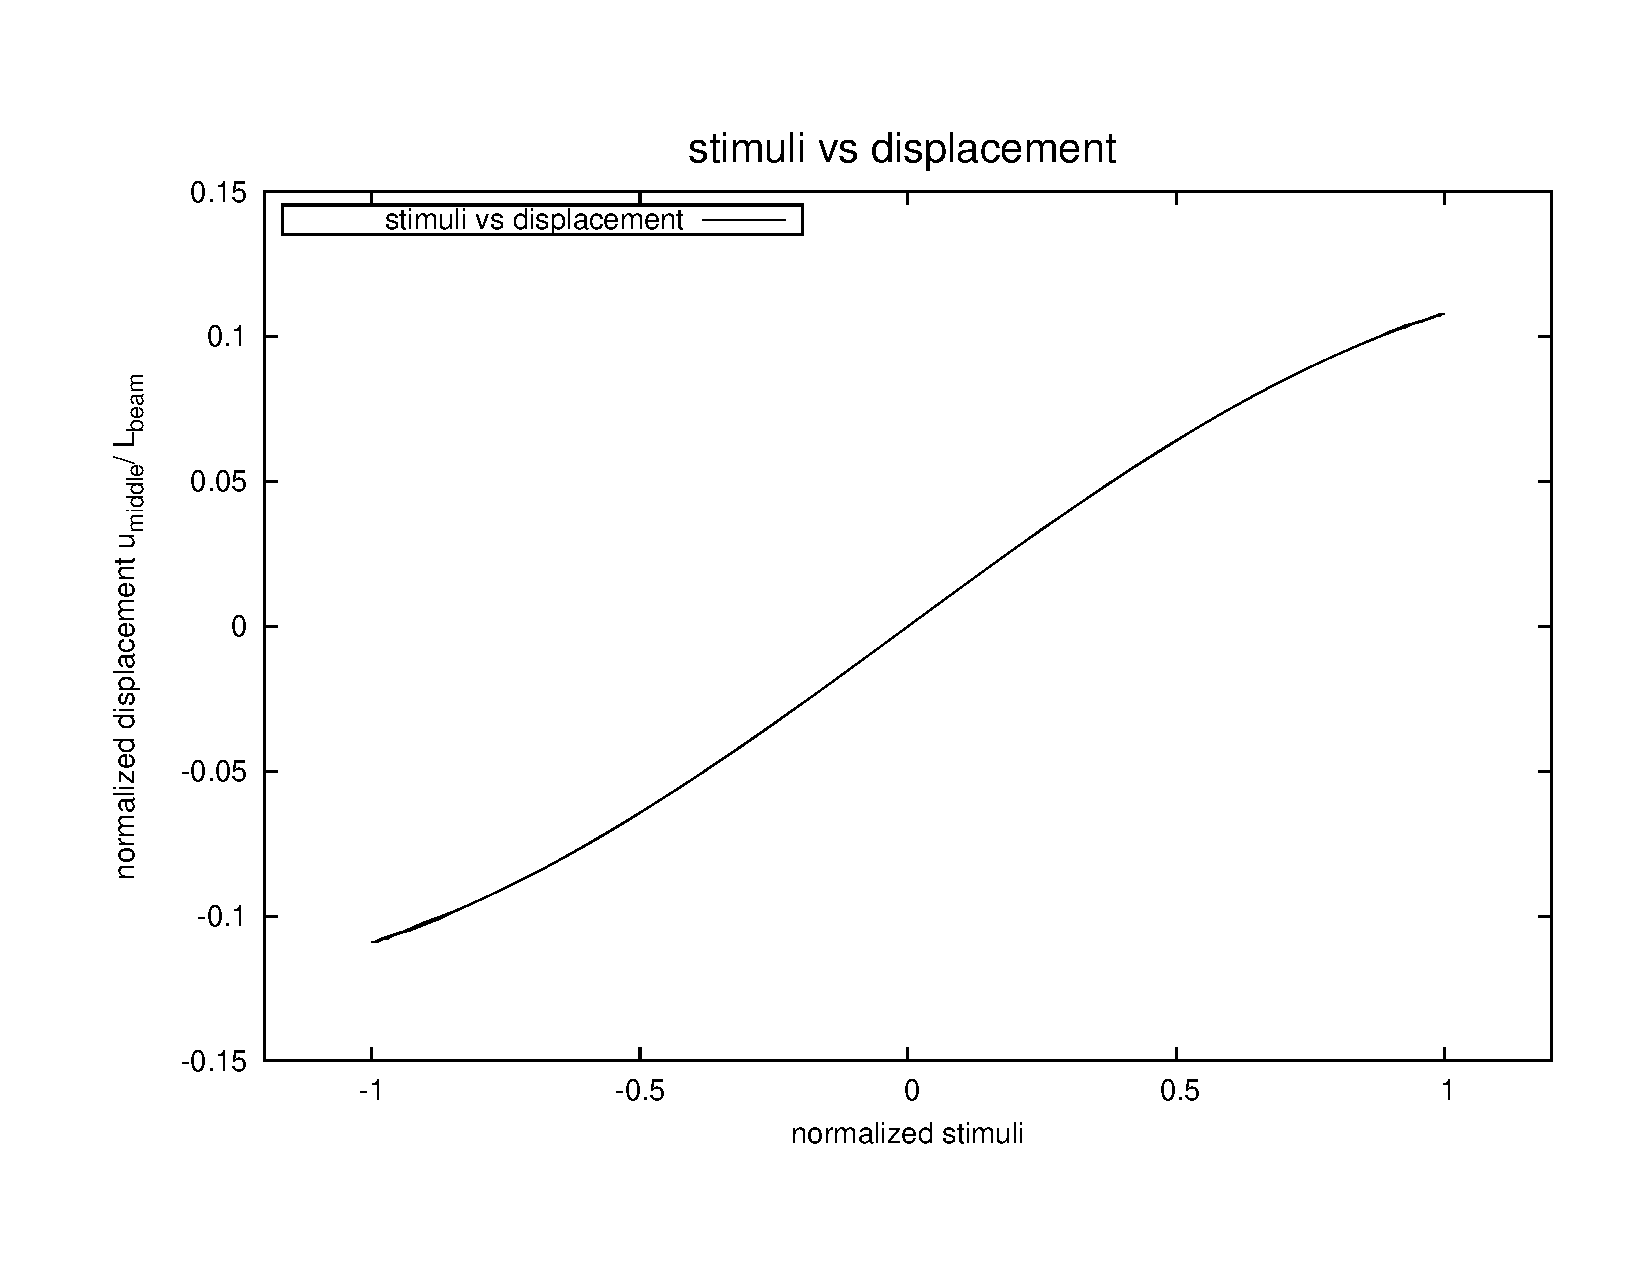
\includegraphics[width=6.0in]{./chap_5_active_trusses/images_non_linear_time_dependent_constitutive_equatio/linear_static_stimuli_vs_displacement.pdf}
\caption{Linear and time independent model for deflection under frequency 1Hz}
\label{fig:linear_static_stimuli_vs_displacement}
\end{figure} 
The nonlinear relationship between the deflection and input stimuli that is shown in figure \ref{fig:linear_static_stimuli_vs_displacement} is mainly due to geometric nonlinearity.

In case the time dependent electro-mechanical response, a cyclic electric field input with frequency 1Hz is prescribed.
The time kernel function with 
$K(t)=1.0-0.6 exp(-t/1.2)$ is considered within the integral representation for the strain 
$\varepsilon_{11}(t)=\int_0^t
K(t-s)\frac{\partial \varepsilon_{11}}{\partial E_3}\frac{\partial
E_3(s)}{\partial s} ds$ 
with 
$\frac{\partial \varepsilon_{11}}{\partial
E_3}=-d_{311}$ 
taken to be 
$340 pm/V$.
The hysteresis between the input stimuli and deflection is shown in figure \ref{fig:linear_tetrahedral_time_dependent_efield_vs_displacement}.

\begin{figure}  
\centering
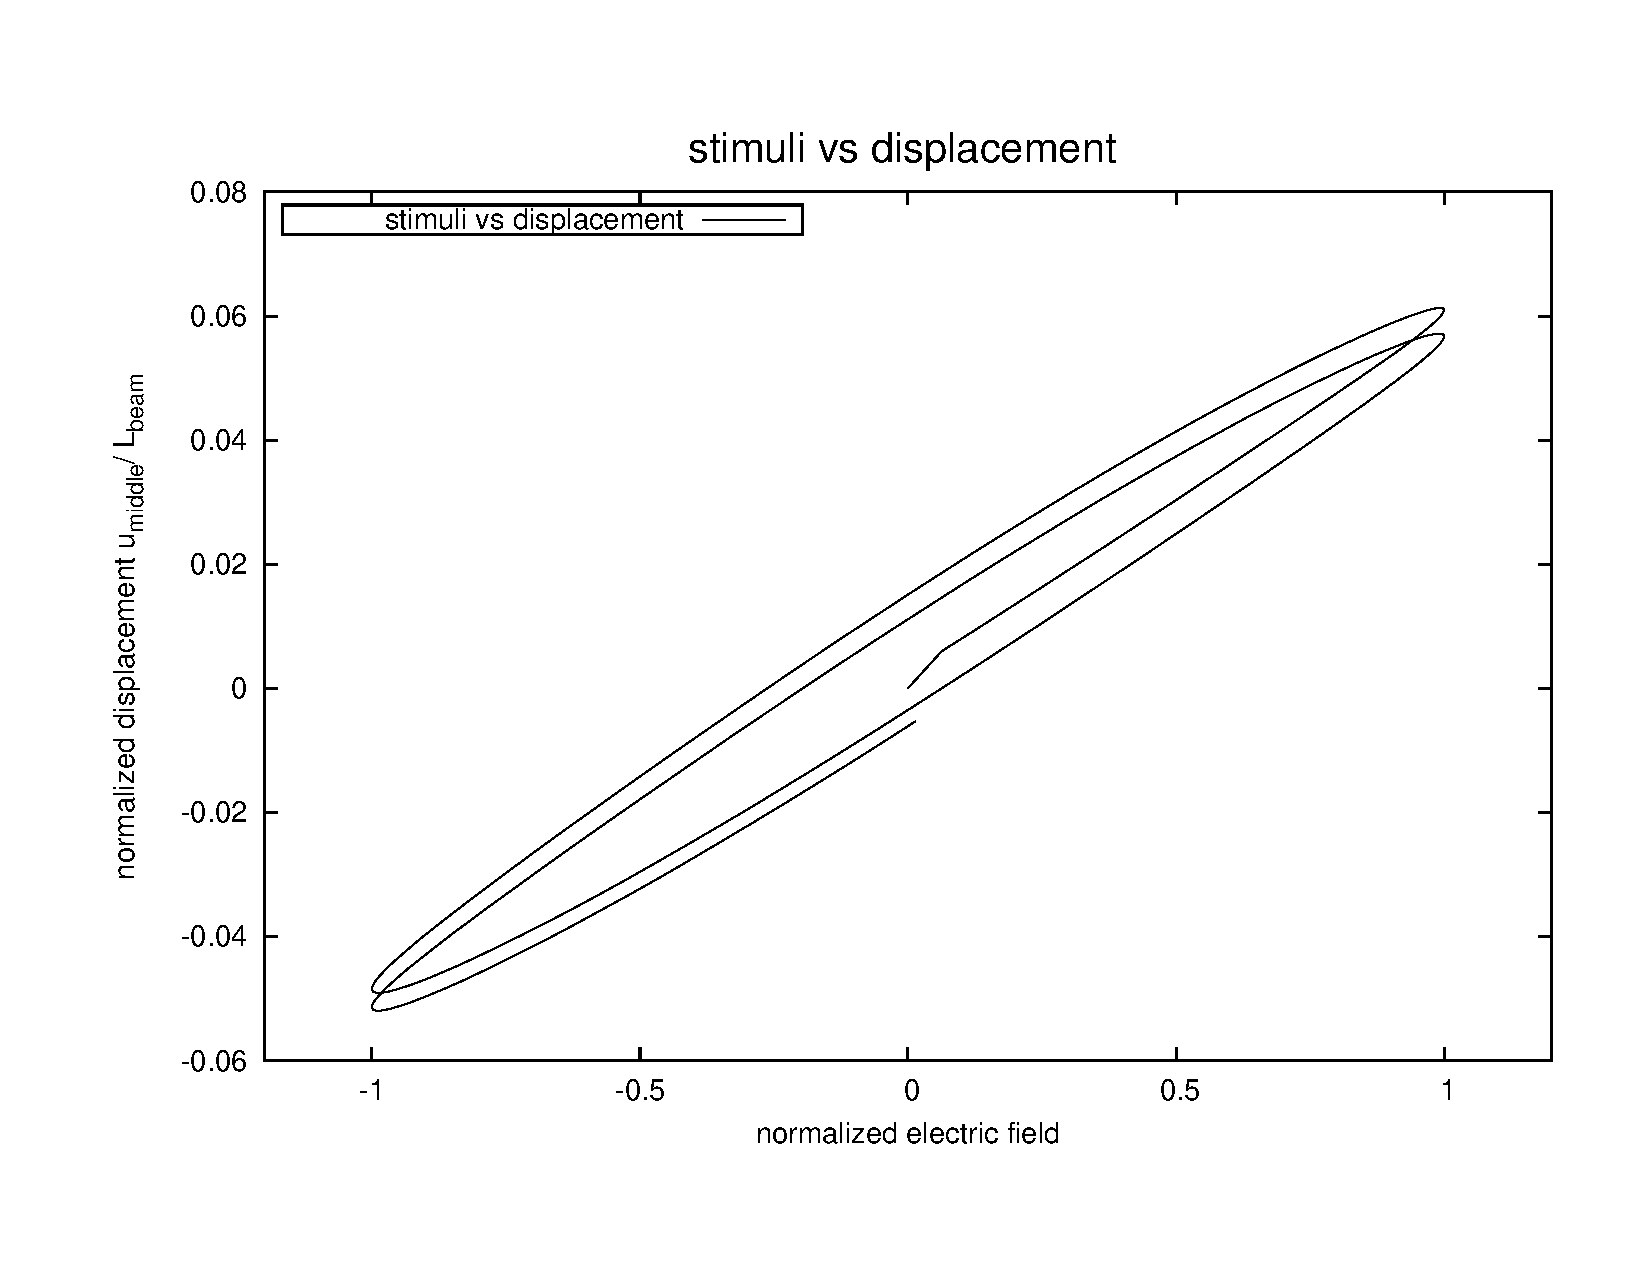
\includegraphics[width=6.0in]{./chap_5_active_trusses/images_non_linear_time_dependent_constitutive_equatio/linear_tetrahedral_time_dependent_efield_vs_displacement.pdf}
\caption{Linear and time dependent response for deflection under frequency 1Hz}
\label{fig:linear_tetrahedral_time_dependent_efield_vs_displacement}
\end{figure} 

We follow the same approach as previous chapters and assume the nonlinear and time dependent response for the constitutive equation in each truss element.
We define a nonlinear response function $\varepsilon_{11}(E_3)=-d_{311}^0 E_3-d_{311}^1 |E_3| E_3$.
Here we take $d_{311}^0=340pm/V$ and\footnote{$f$ here stands for femto i.e. $10^{-15}$ } $d_{311}^1=0.02 fm^2/V^2 $.
The results from taking a nonlinear and time dependent electric coupling between electric stimuli and resulting strain is shown in figure \ref{fig:linear_tetrahedral_time_dependent_efield_vs_displacement_nonlinear}.
The hysteresis curve shown in figure \ref{fig:linear_tetrahedral_time_dependent_efield_vs_displacement_nonlinear} combines the nonlinear response both from the large geometry and also from the nonlinear electro-mechanical constitutive in each truss. 
\begin{figure}   
\centering
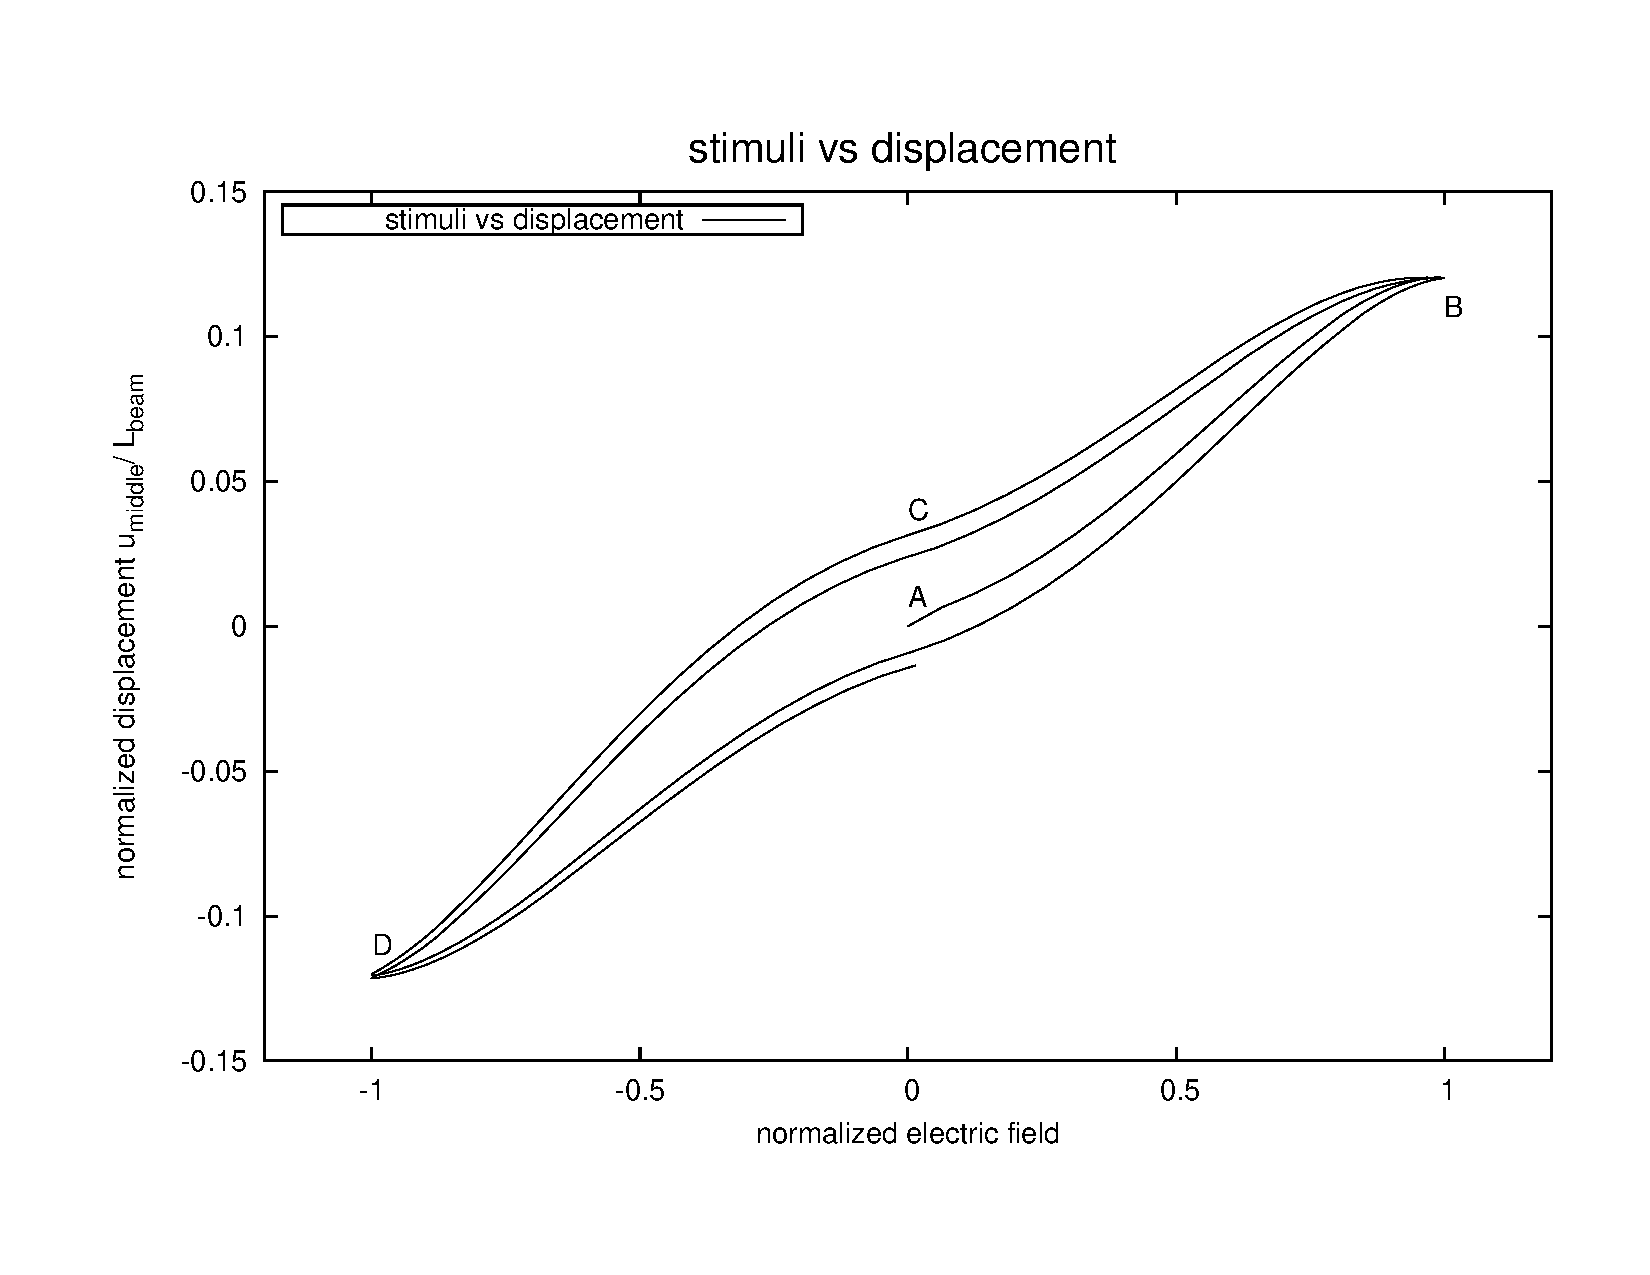
\includegraphics[width=6.0in]{./chap_5_active_trusses/images_non_linear_time_dependent_constitutive_equatio/linear_tetrahedral_time_dependent_efield_vs_displacement_nonlinear.pdf}
\caption{Nonlinear and time dependent response for deflection of beam like truss under frequency 1Hz}
\label{fig:linear_tetrahedral_time_dependent_efield_vs_displacement_nonlinear}
\end{figure} 
In figure \ref{fig:linear_tetrahedral_time_dependent_efield_vs_displacement_nonlinear_snapshot} the configurations of the truss corresponding to four different values of electric stimuli are shown. 


\begin{figure}
\begin{subfigure}{.5\textwidth}
  \centering
  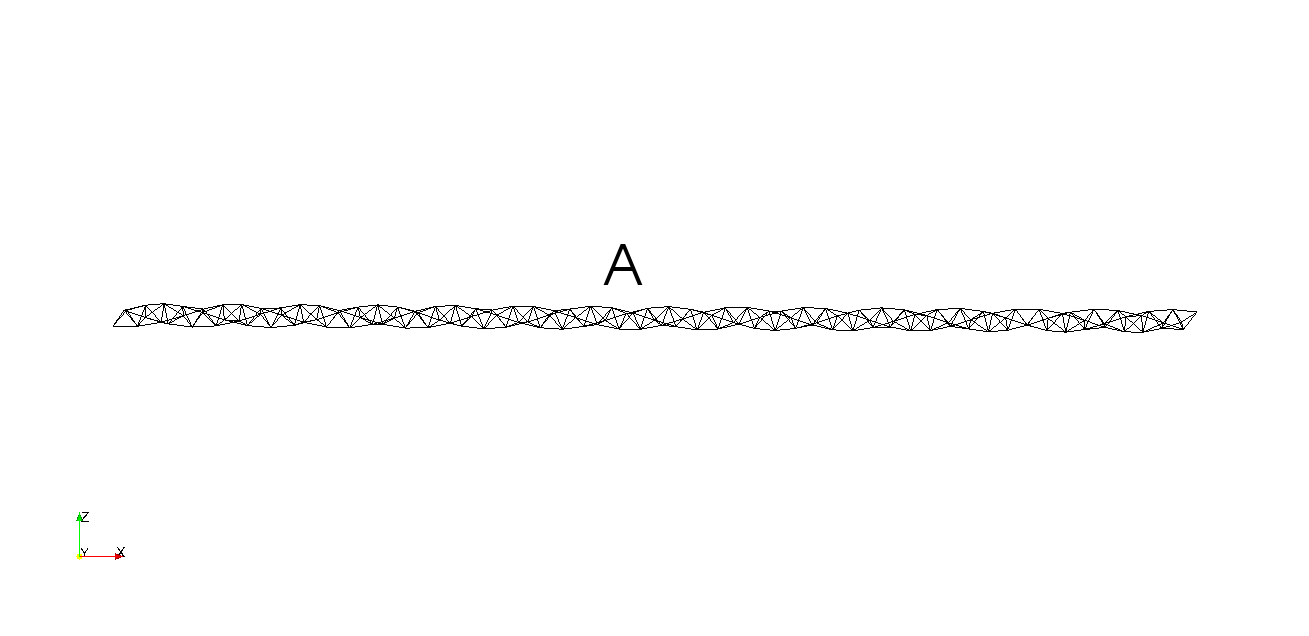
\includegraphics[width=.8\linewidth]{./chap_5_active_trusses/images_non_linear_time_dependent_constitutive_equatio/linear_tetrahedral_bending_snapshop_A.png}  
  \label{fig:sfigA}
\end{subfigure}%
\begin{subfigure}{.5\textwidth}
  \centering
  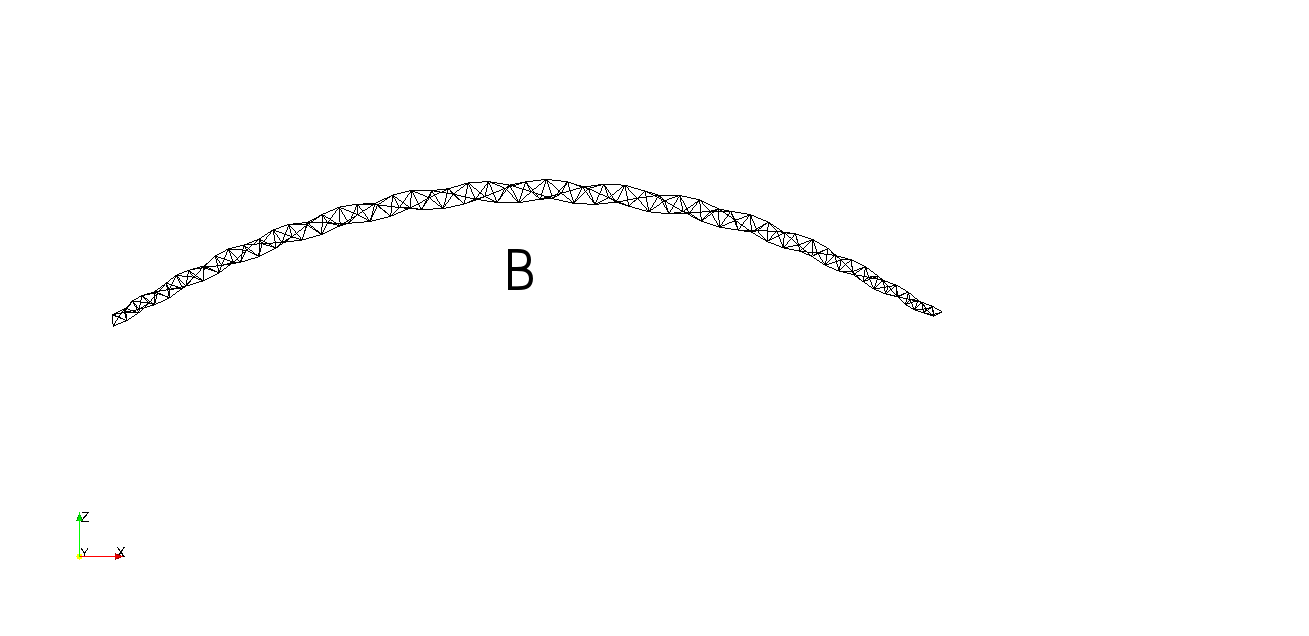
\includegraphics[width=.8\linewidth]{./chap_5_active_trusses/images_non_linear_time_dependent_constitutive_equatio/linear_tetrahedral_bending_snapshop_B.png}
  
  \label{fig:sfigB}
\end{subfigure}

\begin{subfigure}{.5\textwidth} 
  \centering
  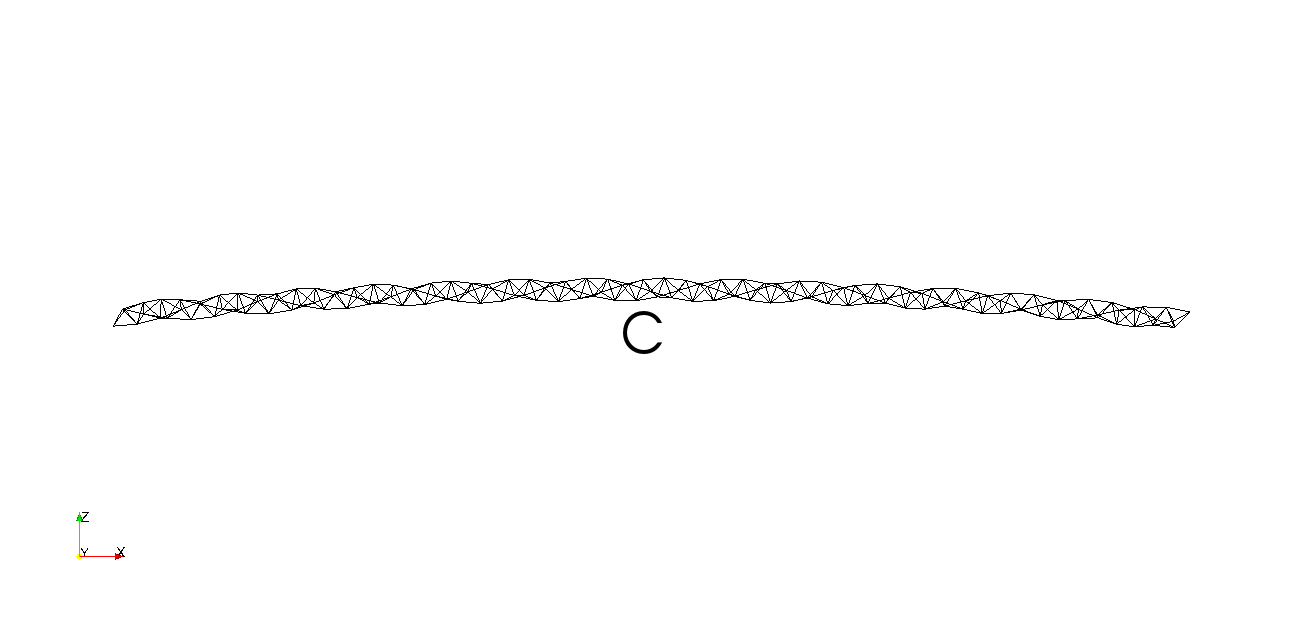
\includegraphics[width=.8\linewidth]{./chap_5_active_trusses/images_non_linear_time_dependent_constitutive_equatio/linear_tetrahedral_bending_snapshop_C.png}
  \label{fig:sfigC}
\end{subfigure}%
\begin{subfigure}{.5\textwidth}
  \centering
  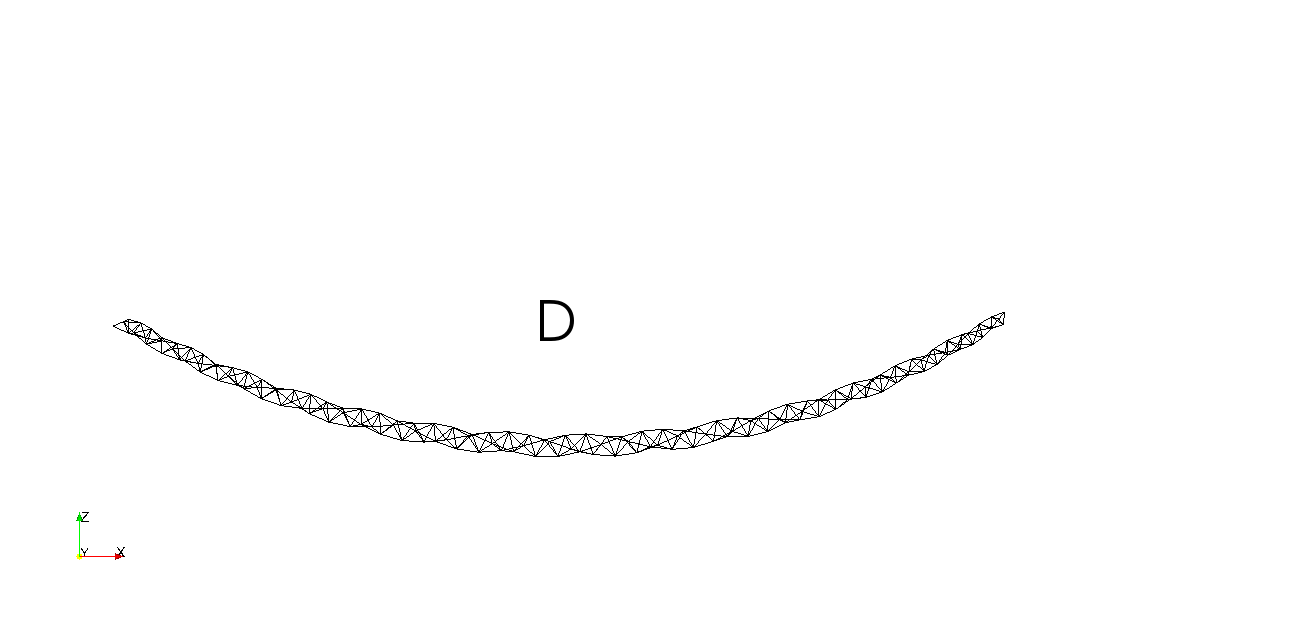
\includegraphics[width=.8\linewidth]{./chap_5_active_trusses/images_non_linear_time_dependent_constitutive_equatio/linear_tetrahedral_bending_snapshop_D.png}
  \label{fig:sfigD}
\end{subfigure}
\caption{The snapshots of linear tetrahedral truss in configurations labeled in figure \ref{fig:linear_tetrahedral_time_dependent_efield_vs_displacement_nonlinear}}
\label{fig:linear_tetrahedral_time_dependent_efield_vs_displacement_nonlinear_snapshot}
\end{figure}


As it can be seen from figures \ref{fig:linear_tetrahedral_bending_strain_contour} and \ref{fig:linear_tetrahedral_bending_efield_contour} the applied strain and therefore electric field can be beyond the limits of material. With a little investigation on the location of the maximum strain, it has been shown that even with the limiting amount of strain it is still possible to get the same shape.

The 1\% strain is chosen as maximum applicable strain.
As a result of limiting strain the resulting shape will change slightly.
The resulting shape with this limiting strain is shown in figure \ref{fig:limiting_strain_linear_tetrahedral_bending_strain_contour}.
Moreover, less electric field will be needed for the actuation as it is shown in figure \ref{fig:limiting_strain_linear_tetrahedral_bending_electric_field_contour}. 
Application of limiting strain in the model will decrease the maximum overall deflection of truss.
This will also change the shape of hysteresis curve as shown in figure  \ref{fig:limiting_strain_linear_tetrahedral_time_dependent_efield_vs_displacement_nonlinear}.

\begin{figure}  
\centering
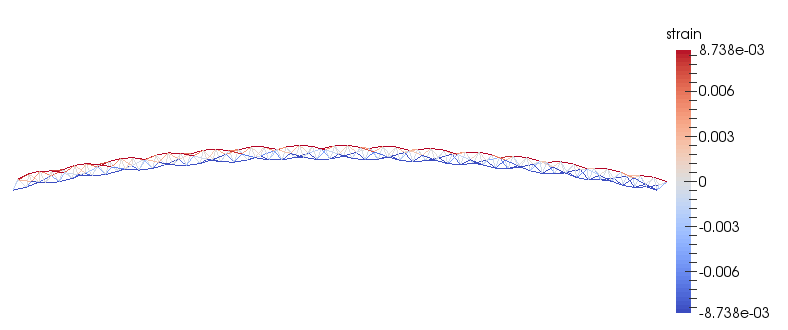
\includegraphics[width=6.0in]{./chap_5_active_trusses/images_non_linear_time_dependent_constitutive_equatio/limiting_strain_linear_tetrahedral_bending_strain_contour.png}
\caption{The strain distribution in a beam like tetrahedral truss in the arc configuration with limiting strain 1\%}
\label{fig:limiting_strain_linear_tetrahedral_bending_strain_contour}
\end{figure} 

\begin{figure}  
\centering
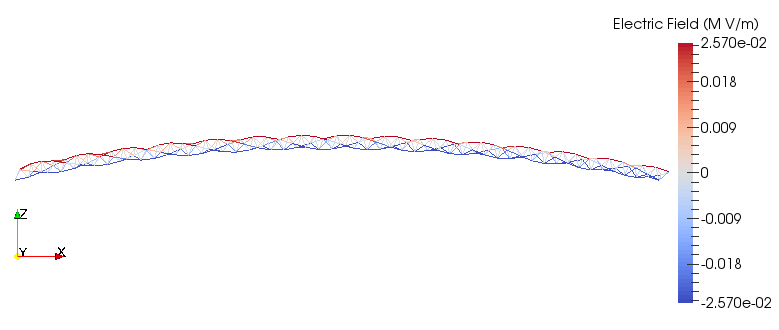
\includegraphics[width=6.0in]{./chap_5_active_trusses/images_non_linear_time_dependent_constitutive_equatio/limiting_strain_linear_tetrahedral_bending_electric_field_contour.png}
\caption{The electric field distribution in a beam like tetrahedral truss in the arc configuration with limiting strain 1\%}
\label{fig:limiting_strain_linear_tetrahedral_bending_electric_field_contour} 
\end{figure} 

\begin{figure}  
\centering
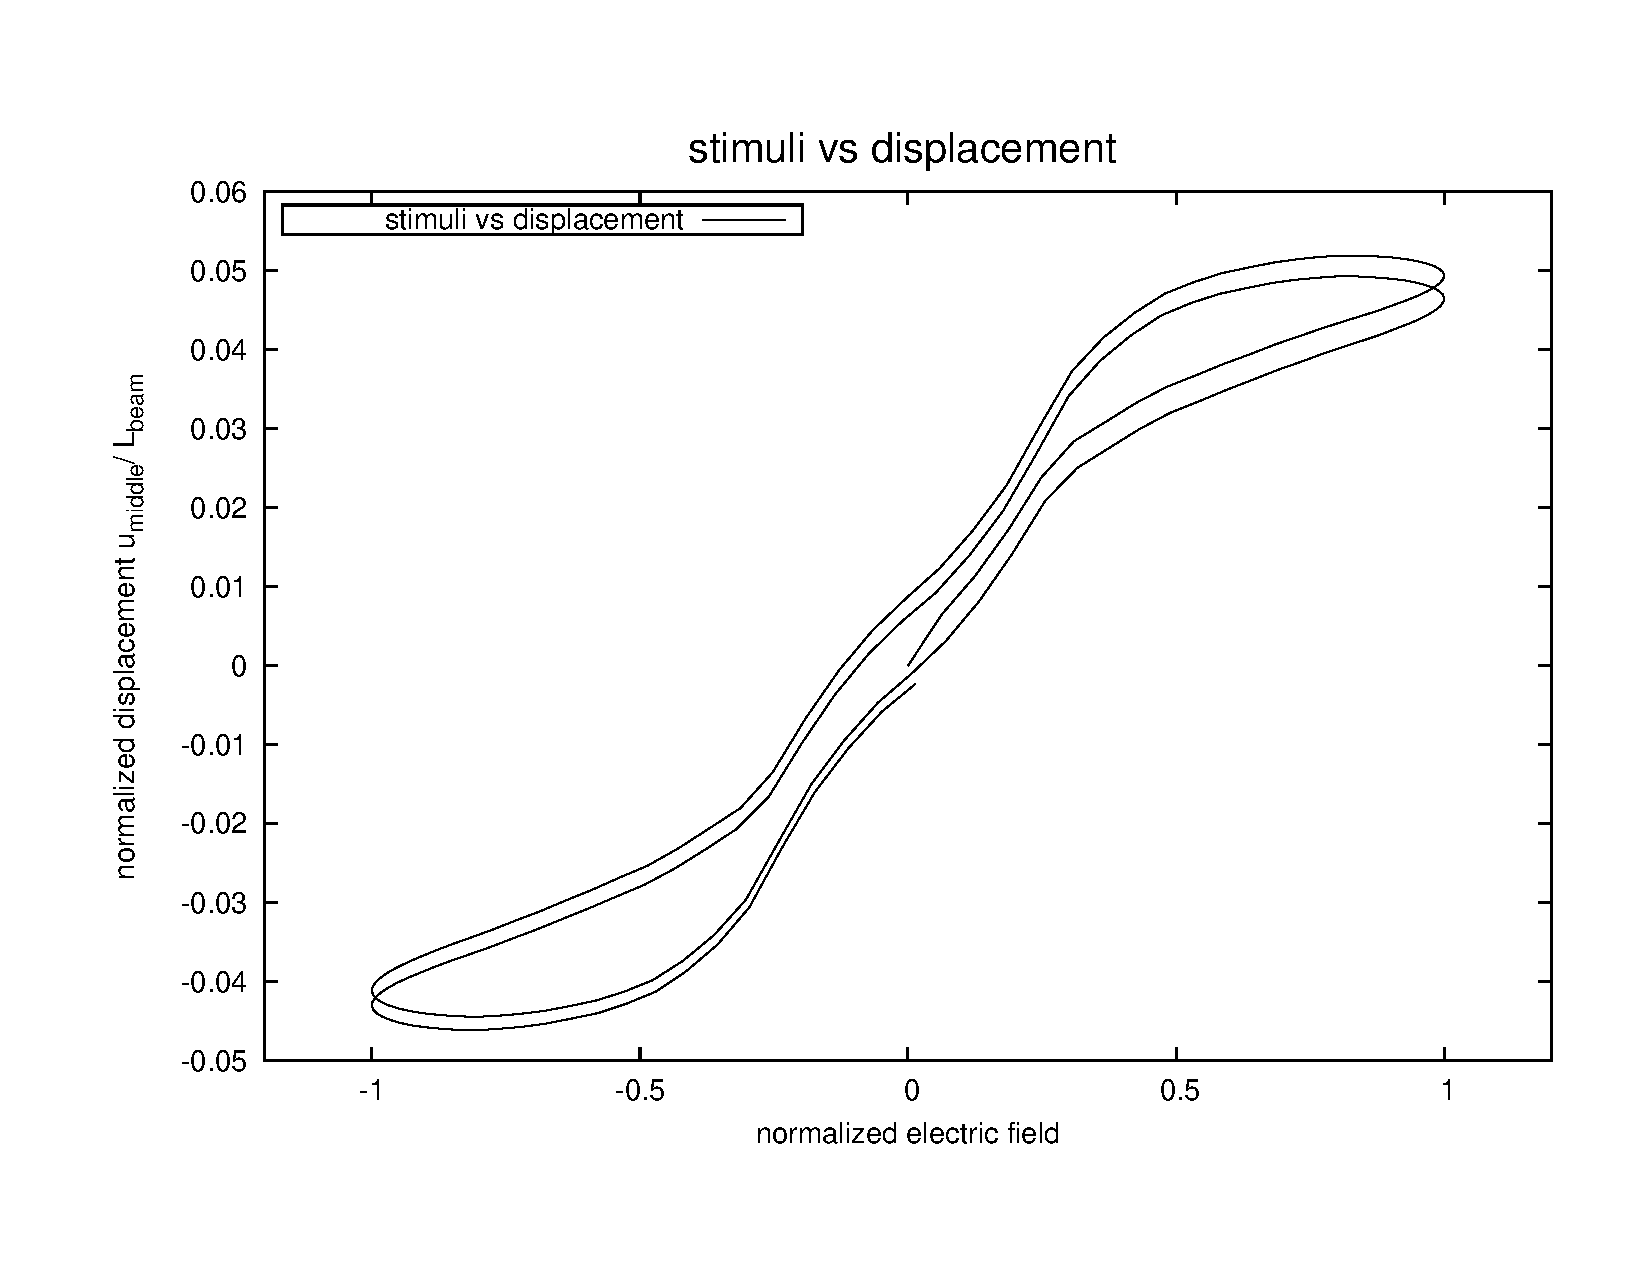
\includegraphics[width=4.0in]{./chap_5_active_trusses/images_non_linear_time_dependent_constitutive_equatio/limiting_strain_linear_tetrahedral_time_dependent_efield_vs_displacement_nonlinear.pdf}
\caption{Nonlinear and time dependent response for deflection of beam like truss under frequency 1Hz with limiting strain}
\label{fig:limiting_strain_linear_tetrahedral_time_dependent_efield_vs_displacement_nonlinear}
\end{figure} 

In order to examine the rate (frequency) dependent response, parametric studies are presented by applying electric fields at various frequencies. Different frequency inputs are applied to the same material constitutive model presented in this section. The corresponding strains response of the truss under different frequencies and amplitudes are shown in figure \ref{fig:truss_linear_Frequency_Effect}. It is apparent from the results that higher frequency of loading reduces time-dependent (hysteresis) effect. This is due to the fact that the material does not have enough time to exhibit time-dependent effect. In higher frequency the response is very similar to the instantaneous responses. 

% Fast loading reduces the creep-like or relaxation-like behavior and the area inside the hysteresis curve becomes smaller.

\begin{figure}
\centering 
\subcaptionbox{Frequency 0.1 Hz} 
{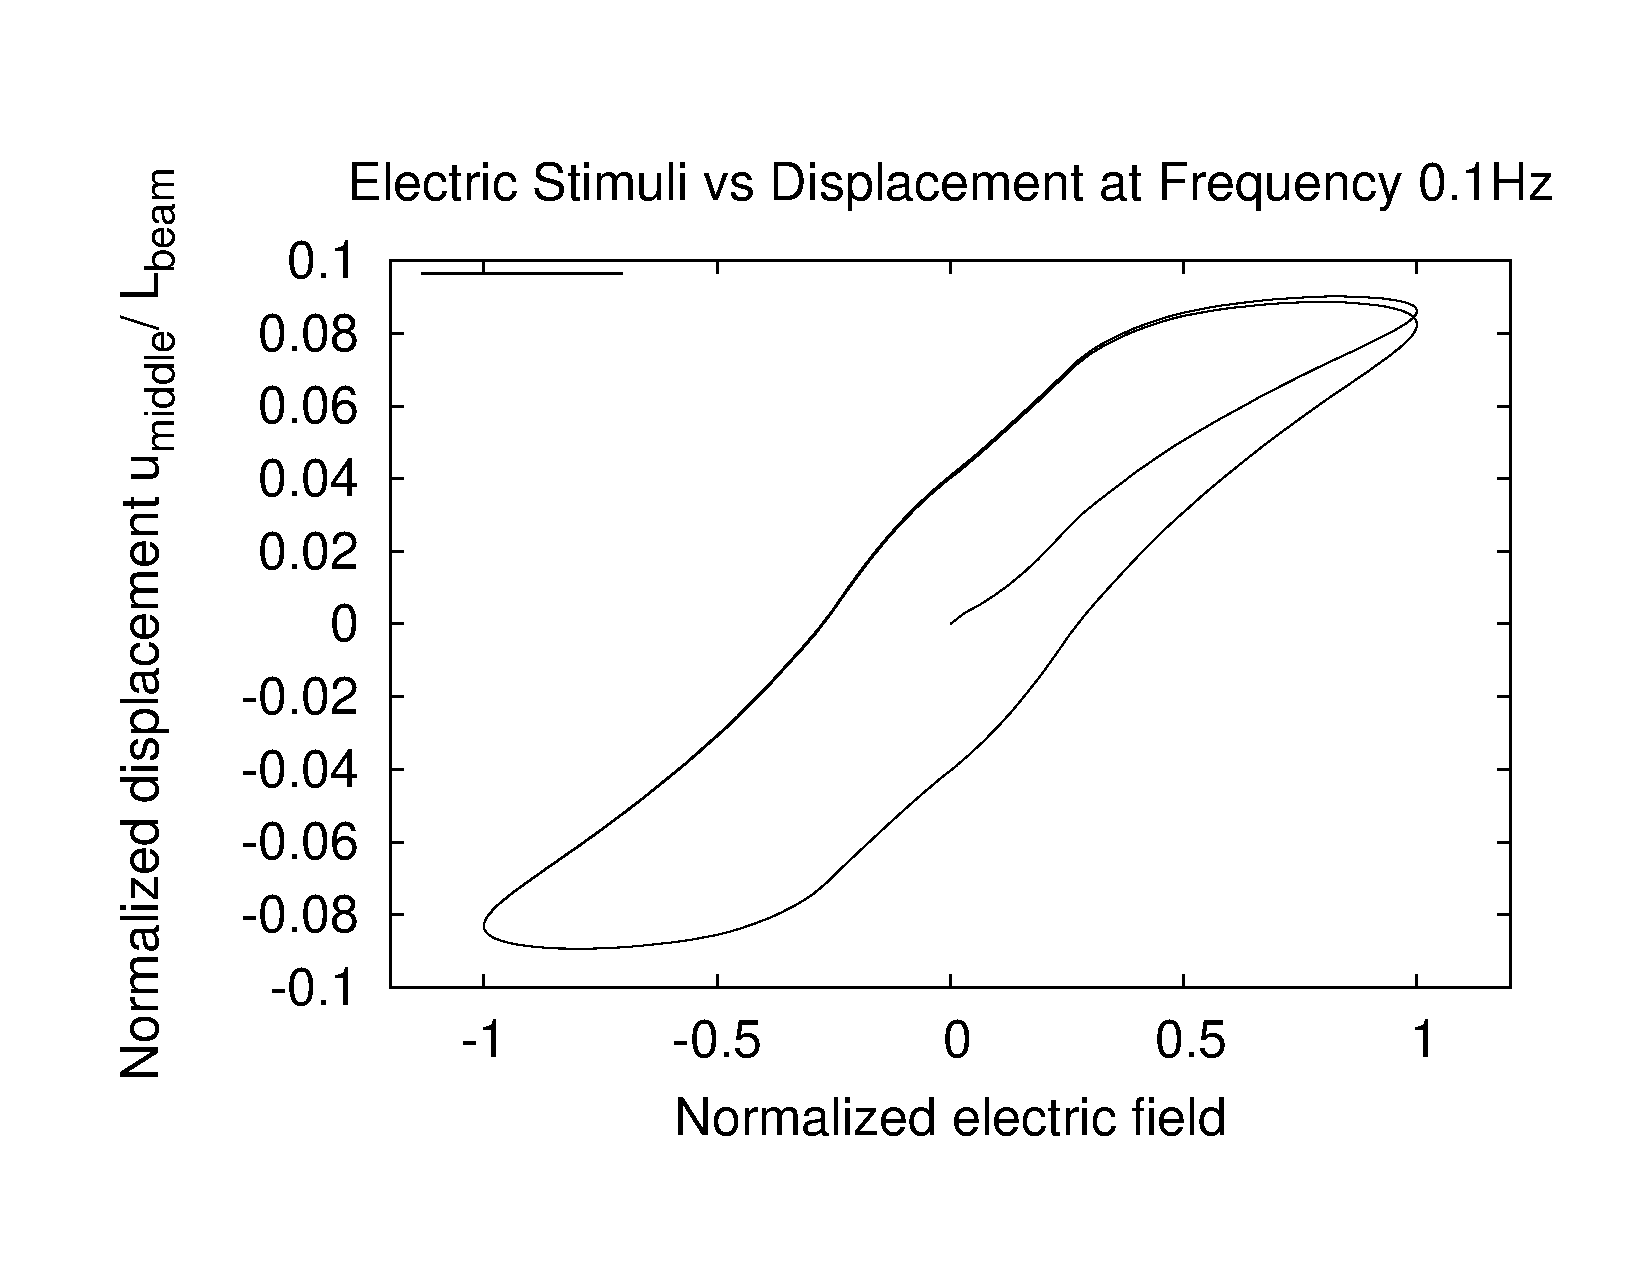
\includegraphics[width=2.9in]{./chap_5_active_trusses/truss_freq_study/truss_nonlinear_freq_0p1.pdf}}
\subcaptionbox{Frequency 0.2 Hz}
{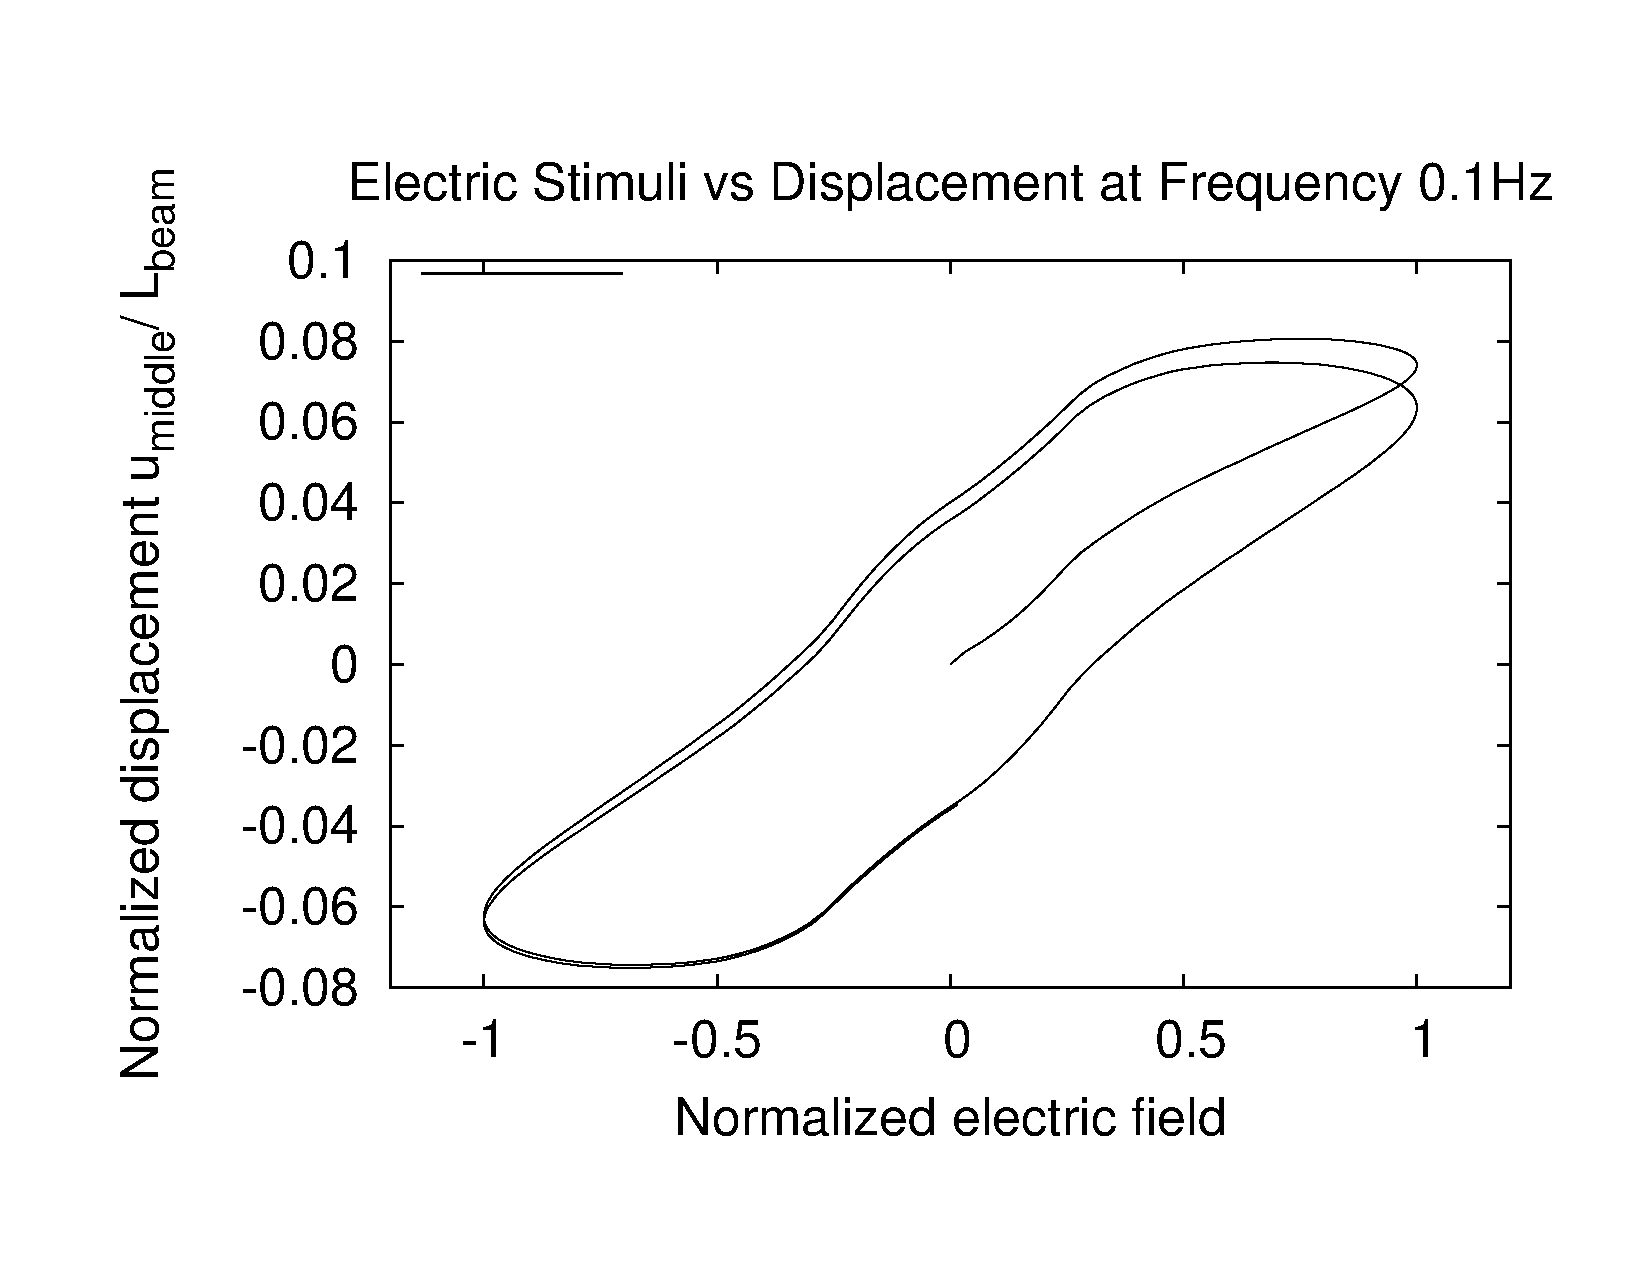
\includegraphics[width=2.9in]{./chap_5_active_trusses/truss_freq_study/truss_nonlinear_freq_0p2.pdf}}
\subcaptionbox{Frequency 0.5 Hz}
{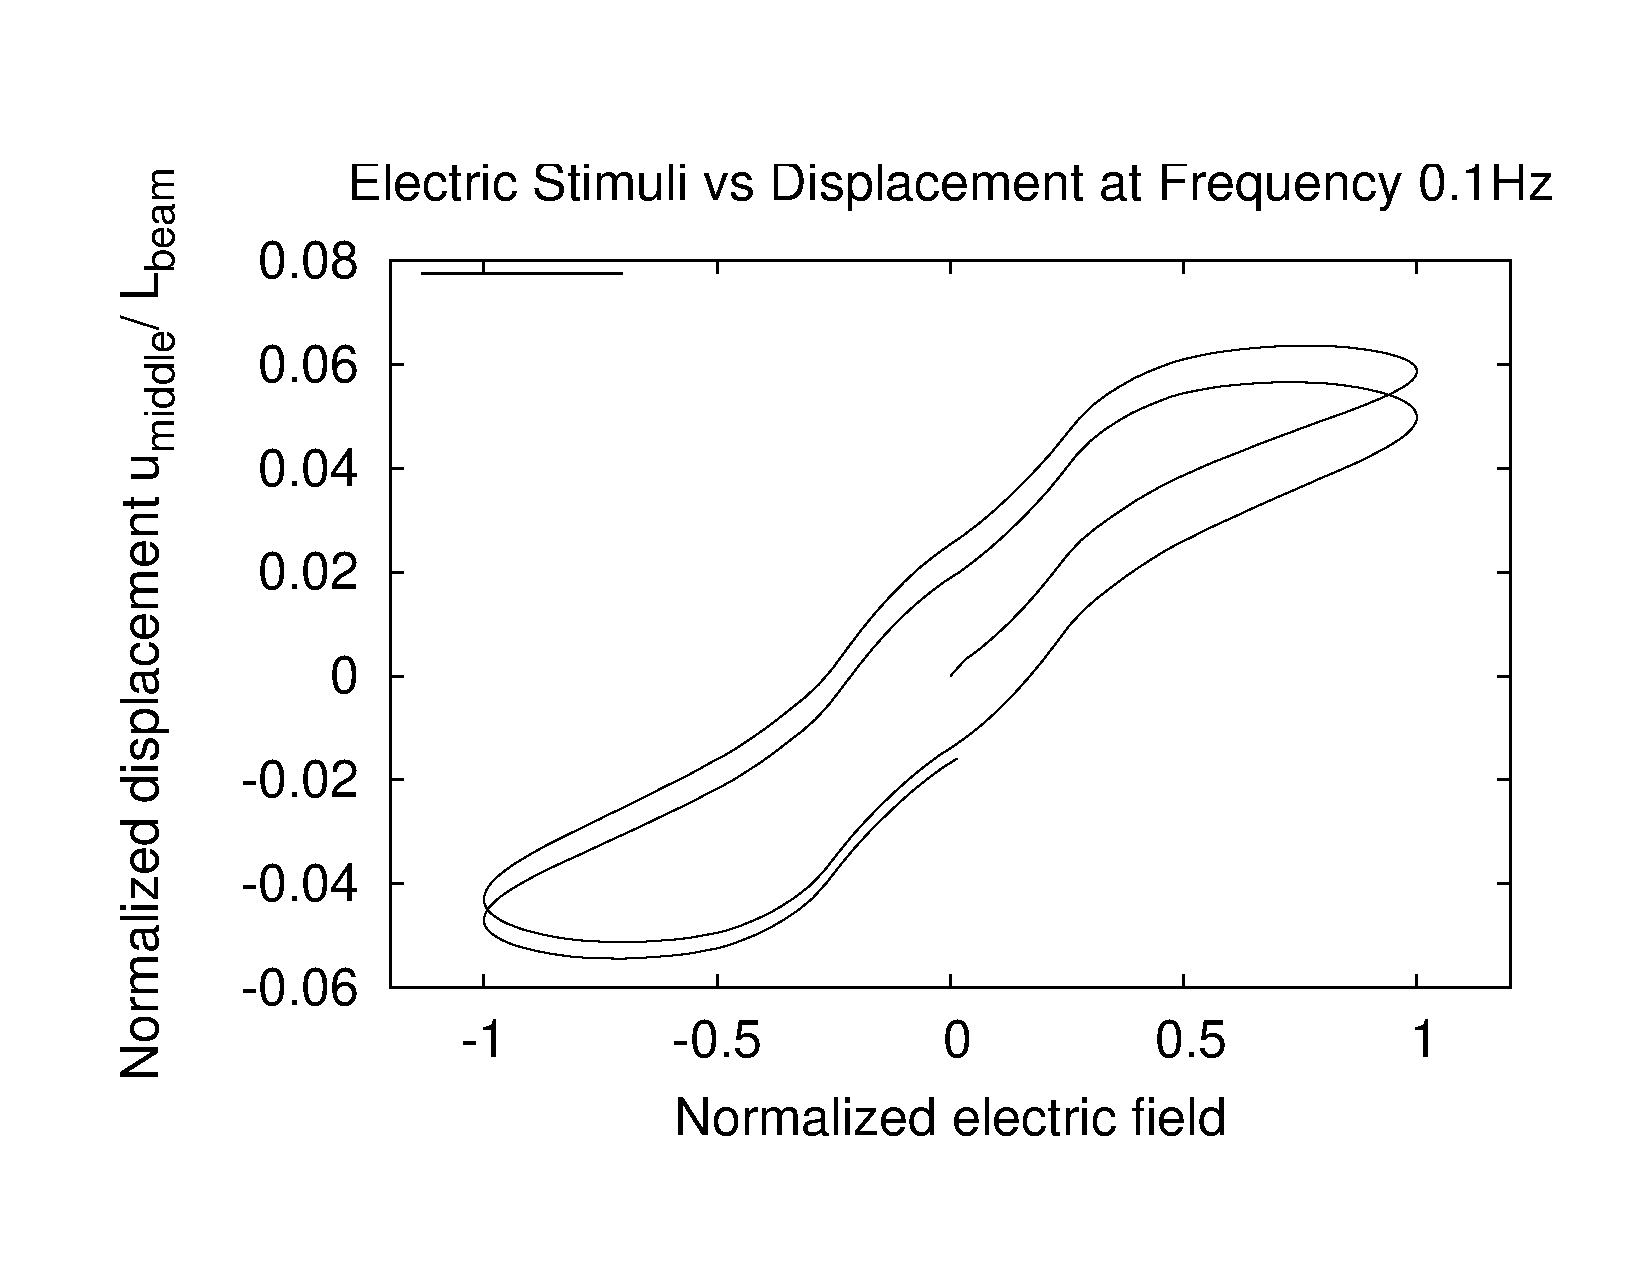
\includegraphics[width=2.9in]{./chap_5_active_trusses/truss_freq_study/truss_nonlinear_freq_0p5.pdf}}
\subcaptionbox{Frequency 2.0 Hz}
{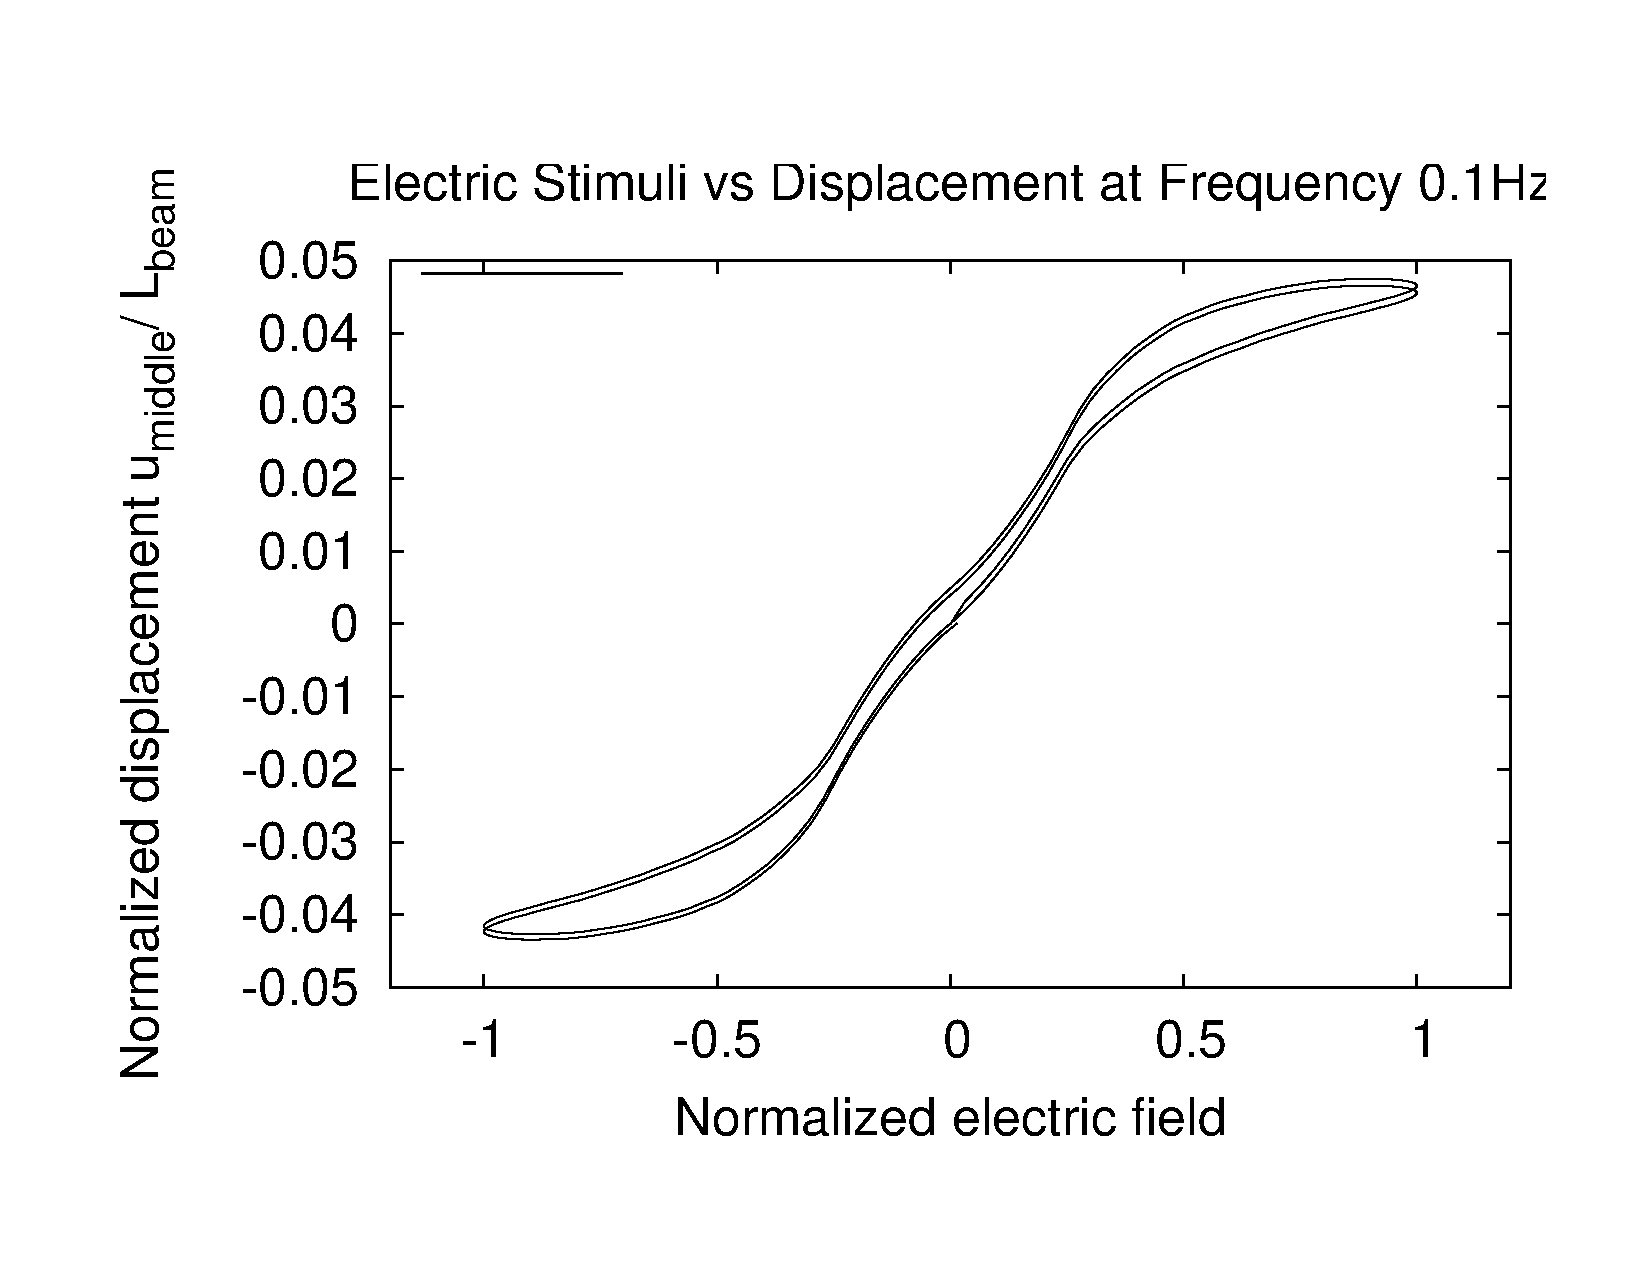
\includegraphics[width=2.9in]{./chap_5_active_trusses/truss_freq_study/truss_nonlinear_freq_2p0.pdf}}
\subcaptionbox{Frequency 5.0 Hz}
{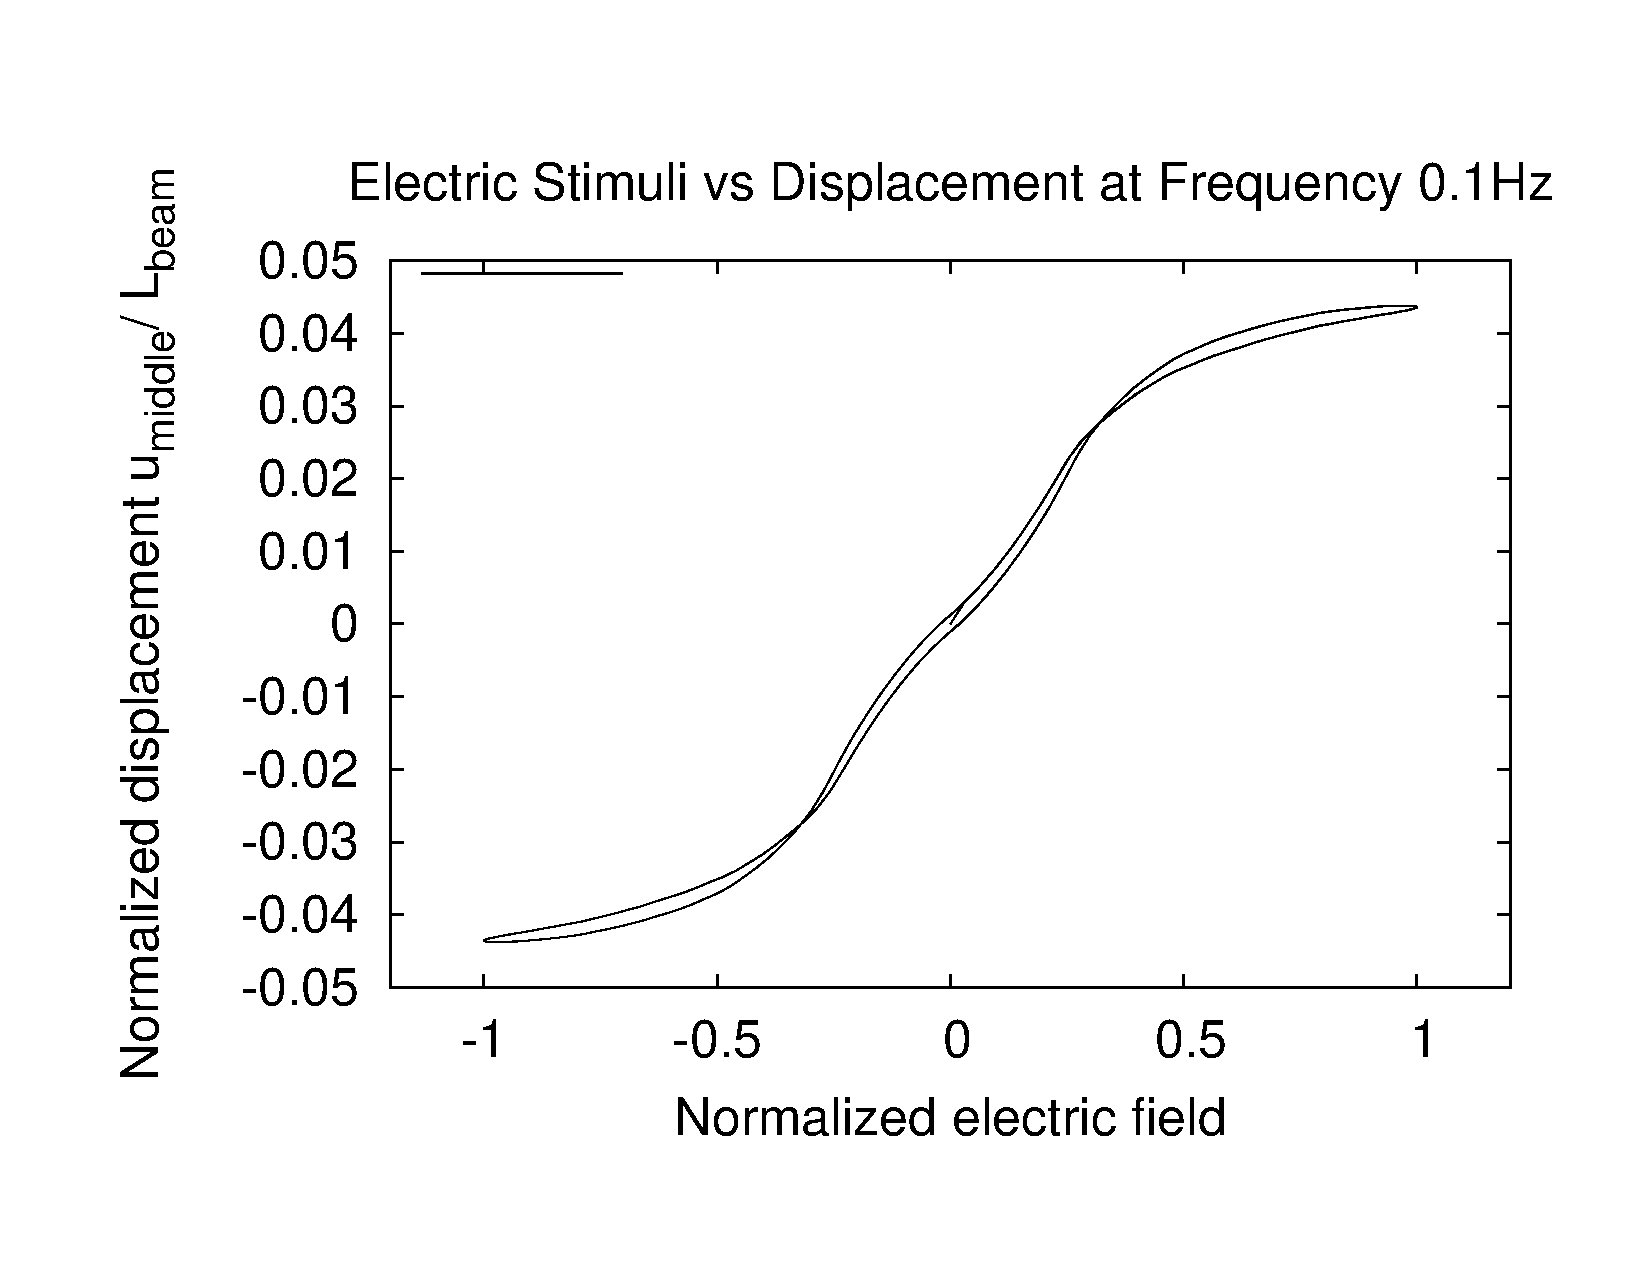
\includegraphics[width=2.9in]{./chap_5_active_trusses/truss_freq_study/truss_nonlinear_freq_5p0.pdf}}
\subcaptionbox{Frequency 10.0 Hz}
{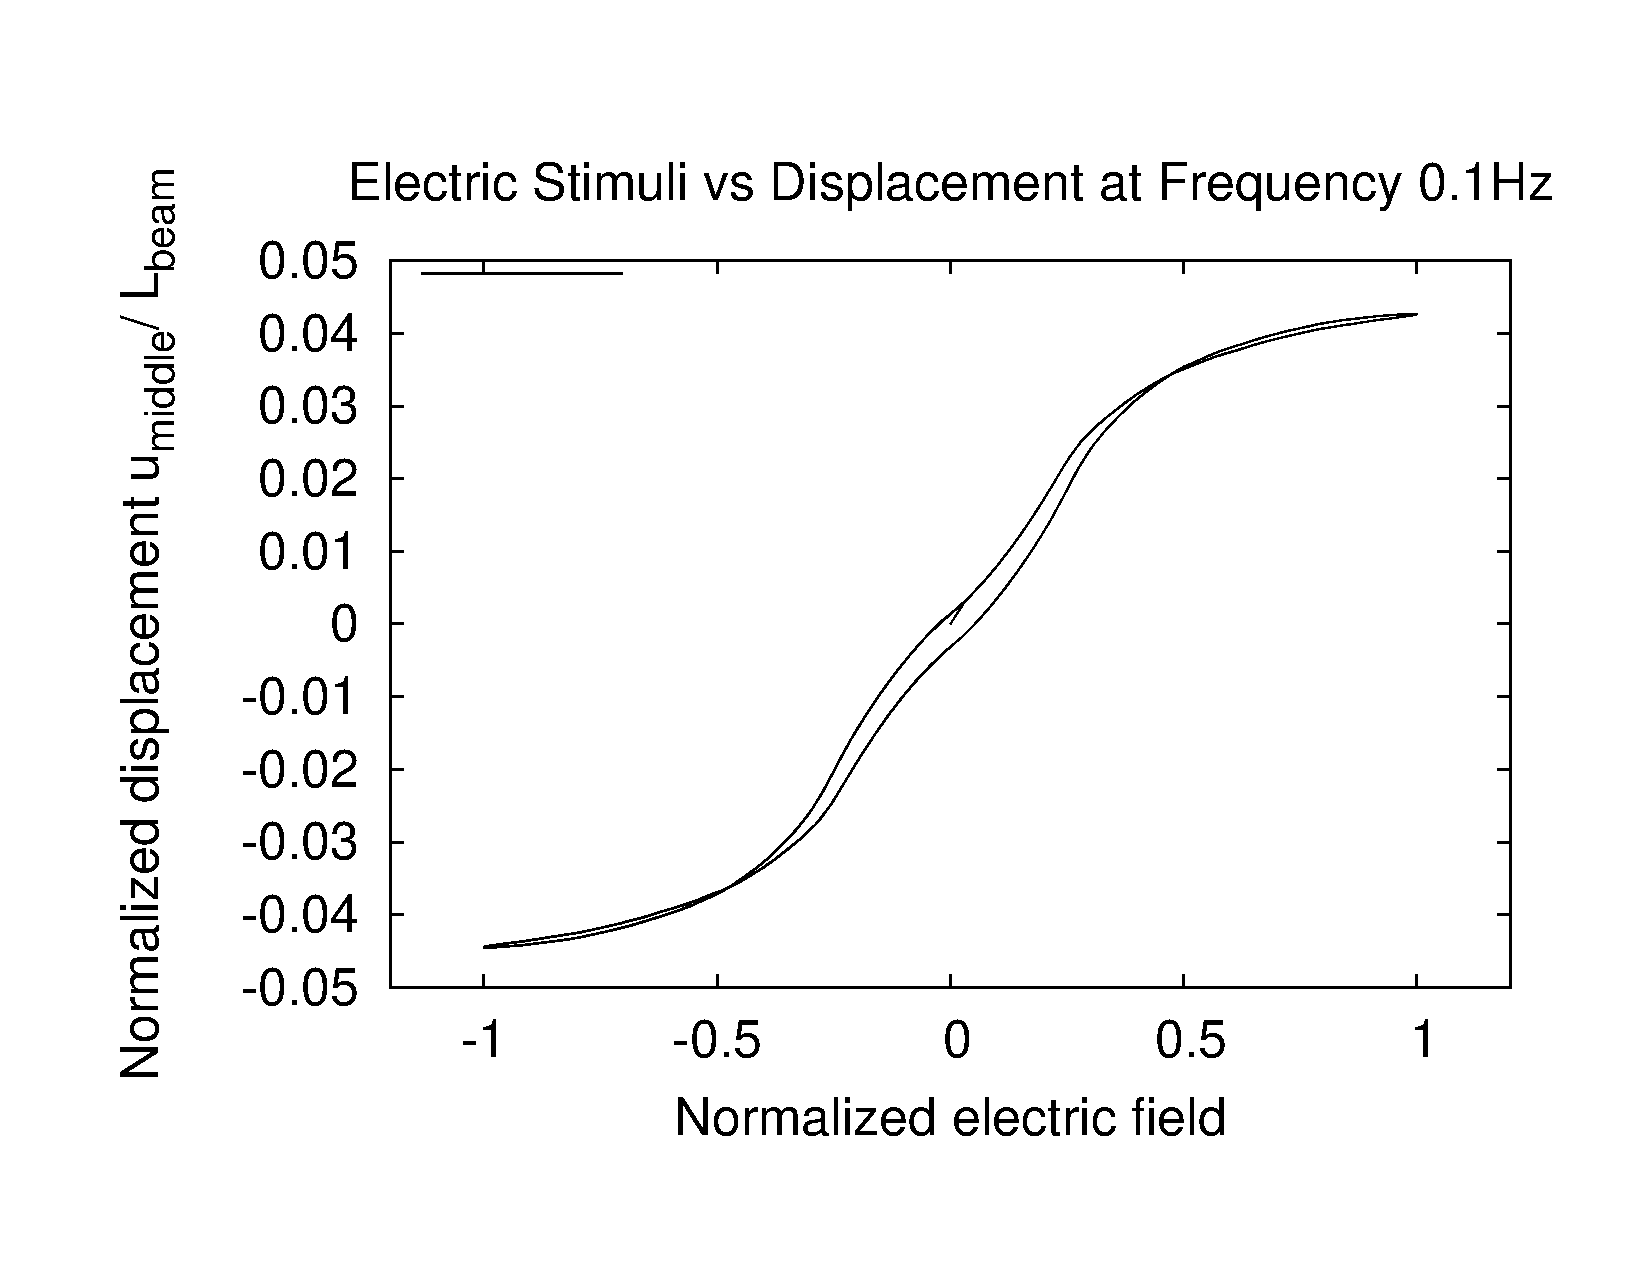
\includegraphics[width=2.9in]{./chap_5_active_trusses/truss_freq_study/truss_nonlinear_freq_10p0.pdf}}
\caption{Effect of frequency of applied electric field on strain response of tetrahedral truss}
\label{fig:truss_linear_Frequency_Effect}
\end{figure}